\chapter{Results}
\label{chap:results}

This chapter begins with a description of the experimental setup and key assumptions. We then give a brief overview of the dataset. The main section evaluates and compares different versions of our model, focusing on how each added component affects performance. Finally, we explore how the model's performance depends on the number of training experiments.

To simplify notation throughout this chapter, we use the following abbreviations for the model layers: X\_ON and X\_OFF represent the LGN ON and OFF cell populations. V1\_Exc\_L4 and V1\_Inh\_L4 refer to the excitatory and inhibitory cell populations in V1 layer 4, and V1\_Exc\_L23 and V1\_Inh\_L23 refer to those in V1 layer 2/3. These match the layer names used in our model code and will be used consistently throughout.

\section{Experimental Setup and Technicalities}
\label{sec:experimental_setup}

Unless otherwise specified, all experiments were run using the model setup and artificial dataset described in Chapter~\ref{chap:methods}.

In addition to the setup from the previous chapter, we used several parameters chosen based on our experience during model development. These were mostly influenced by practical constraints such as limited GPU access, memory availability, or model-specific issues. Because thorough testing of all parameter combinations would have required too many resources, we selected values that we believed were reasonable. While we do not expect these parameters to drastically affect our findings, they could be optimized in future work.

ne important parameter is the batch size. As explained in Section~\ref{sec:artificial_dataset}, our dataset is made up of samples that each represent a single experiment. These had to be grouped into batches for training. We chose a batch size of $50$ based on a balance of performance and hardware limits. Training RNNs on time-based data is typically slow, since computations must happen in sequence and cannot be easily parallelized. Using larger batch sizes allows some parallel processing on GPUs, which helps speed things up. However, larger batches also require more memory.

Memory demands were particularly high when using certain RNN neuronal modules, described in Section~\ref{subsec:additional_modules}, that rely on truncated backpropagation through time (TBPTT). TBPTT increases memory use significantly, especially when paired with small shared neural networks used in place of typical activation functions. To reduce this load, we merged time bins into 20~ms intervals, as described in Section~\ref{subsubsec:time_bins_merging}, which helped but did not fully solve the issue. As noted in Section~\ref{subsubsec:subset_selection}, we also had to limit our model to just 10\% of the artificial neurons from each layer of the original SNN template to stay within memory limits. After weighing all these factors, we chose a batch size of $50$, which worked reliably even with the most memory-intensive versions of our model, like the one using the synaptic depression module (Section~\ref{subsubsec:synaptic_depression}).

Another training safeguard we used was gradient clipping, which prevents gradients from growing too large and causing numerical issues. In all our experiments, we clipped gradients to a maximum value of 10,000. This was mainly a precaution to avoid overflow errors during training, especially during early development phases when we were experimenting with activation functions other than LeakyTanh. This topic is discussed further in Section~\ref{subsubsec:leakytanh}. In our final models, this gradient clipping had little to no effect on performance, but we kept it in place to ensure stability.

Finally, we want to mention the hardware used to run our experiments. Most were carried out on the Metacentrum computing cluster. While not every model variant needed a large GPU, we generally used GPUs with at least 40~GB of RAM. These are well-suited for deep learning tasks and were essential for models that relied on TBPTT. We also used machines with at least 8 CPU cores and 100~GB of RAM to support the computational load.


\section{Dataset Overview}
\label{sec:dataset_overview}

In this section, we present a statistical analysis of our dataset and evaluate the impact of the dataset simplifications we applied. First, we assess the effect of merging time bins from 1~ms to 20~ms, followed by an analysis of the influence of selecting a random subset comprising 10\% of neurons. All scripts used for this analysis are provided in the supplementary materials and the project's GitHub repository.

\subsection{Time Bin Merging Analysis}
\label{subsec:time_bin_merging_analysis}
As described in Section~\ref{subsubsec:time_bins_merging}, we merged the original 1~ms time bins into 20~ms intervals to accelerate computation and reduce data noisiness, while maintaining sufficient temporal resolution. We performed experiments using five bin sizes: 1~ms, 5~ms, 10~ms, 15~ms, and 20~ms. Due to the high computational cost of reprocessing the dataset for each binning size, we limited the analysis to this subset. Each configuration required substantial memory for processing and storage, which constrained the number of variants we could feasibly evaluate. The binning was introduced to significantly accelerate model training and reduce memory consumption.

\subsubsection{Total Spike Counts Across Time Bins}
\label{subsubsec:spike_counts_time_bins}

We begin by comparing the distribution of spike counts across all time bins for each binning size. We hypothesize the following:

\begin{claim}[Distribution of Spike Counts Across All Time Bins]
    The distribution of spike counts across time bins remains similar for bin sizes \{1, 5, 10, 15, 20\}~ms. This suggests that the temporal behavior of neuronal responses is largely preserved.
\end{claim}
\label{claim:tim_bin_counts}

Our assumption is that maintaining the binary-like properties of spike data should also preserve its temporal characteristics. Tables~\ref{tab:train_bin_count_distribution} and~\ref{tab:test_bin_count_distribution} show spike count distributions for the training and test datasets, respectively.

\begin{table}
    \centering\footnotesize\sf
    \begin{tabular}{cccccc}
    \toprule
        Spike Count & 1 ms & 5 ms & 10 ms & 15 ms & 20 ms \\
        \midrule
        0 & 0.9944 & 0.9727 & 0.9491 & 0.9287 & 0.9105 \\
        1 & 0.0056 & 0.0266 & 0.0460 & 0.0598 & 0.0710 \\
        2 & 0.0000 & 0.0007 & 0.0046 & 0.0100 & 0.0147 \\
        3 & 0.0000 & 0.0000 & 0.0003 & 0.0013 & 0.0032 \\
        4 & 0.0000 & 0.0000 & 0.0000 & 0.0001 & 0.0005 \\
        5 & 0.0000 & 0.0000 & 0.0000 & 0.0000 & 0.0001 \\
    \addlinespace % a nice non-intrusive separator of data groups (or final table sums)
    \bottomrule
    \end{tabular}
    \caption{\textbf{Spike count distribution in the train dataset:} This table shows the proportion of time bins containing 0 to 5 spikes for different time bin sizes. Spike counts above 5 are omitted as they occur rarely and have a negligible impact on the overall distribution.}
    \label{tab:train_bin_count_distribution}
\end{table}
    

\begin{table}
    \centering\footnotesize\sf
    \begin{tabular}{cccccc}
    \toprule
        Spike Count & 1 ms & 5 ms & 10 ms & 15 ms & 20 ms \\
    \midrule
        0 & 0.9944 & 0.9728 & 0.9493 & 0.9290 & 0.9107 \\
        1 & 0.0056 & 0.0265 & 0.0458 & 0.0597 & 0.0710 \\
        2 & 0.0000 & 0.0007 & 0.0045 & 0.0099 & 0.0146 \\
        3 & 0.0000 & 0.0000 & 0.0003 & 0.0013 & 0.0032 \\
        4 & 0.0000 & 0.0000 & 0.0000 & 0.0001 & 0.0005 \\
        5 & 0.0000 & 0.0000 & 0.0000 & 0.0000 & 0.0001 \\
    \addlinespace % a nice non-intrusive separator of data groups (or final table sums)
    \bottomrule
    \end{tabular}
    \caption{\textbf{Spike count distribution in the test dataset:} This table shows the proportion of time bins containing 0 to 5 spikes for different time bin sizes. Spike counts above 5 are omitted as they occur rarely and have a negligible impact on the overall distribution.}
    \label{tab:test_bin_count_distribution}
\end{table}

The distributions for both training and test sets are highly similar. Most time bins contain either zero or one spike, and only a small proportion include more than one. For the 20~ms bins, about 1.5\% of time bins contain two or more spikes. Notably, the percentage of time bins with at least one spike increases from roughly 0.6\% (1~ms bins) to 7\% (20~ms bins). This reduction in sparsity supports the hypothesis that the 20~ms bin size offers a reasonable balance between temporal resolution and data density.

Figures~\ref{fig:spike_count_distribution_train} and~\ref{fig:spike_count_distribution_test} further illustrate this by showing spike count distributions across all neuronal populations.

\begin{figure}
    \centering
    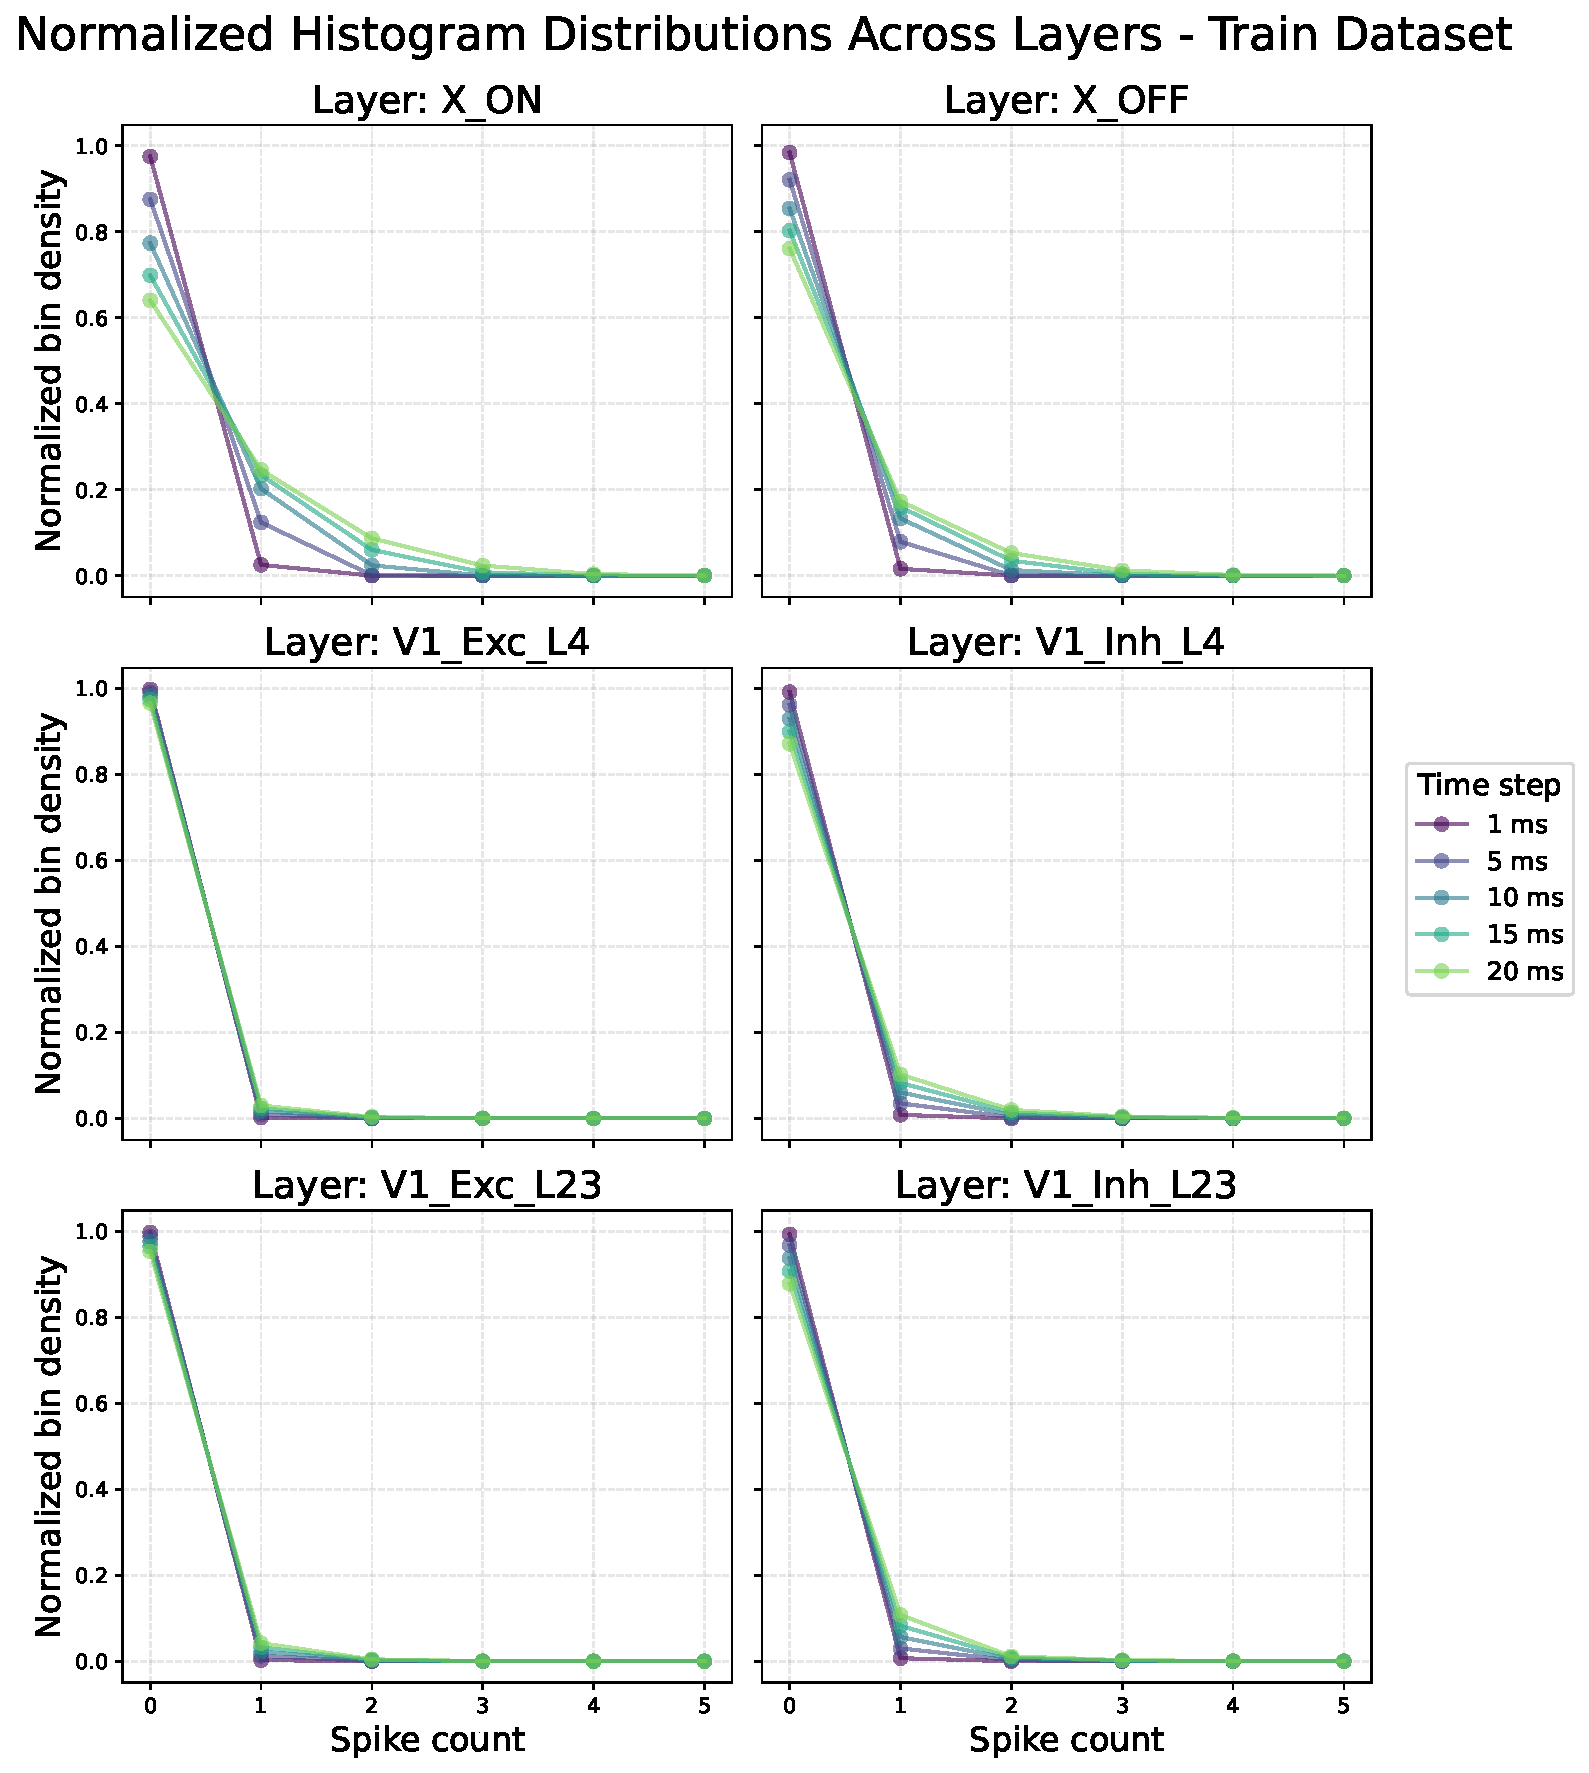
\includegraphics[width=\linewidth]{img/plots/time_step_counts_train.pdf}
    \caption{Evolution of spike counts per time bin with increasing bin size across all neuronal populations in the train dataset.}
    \label{fig:spike_count_distribution_train}
\end{figure}

\begin{figure}
    \centering
    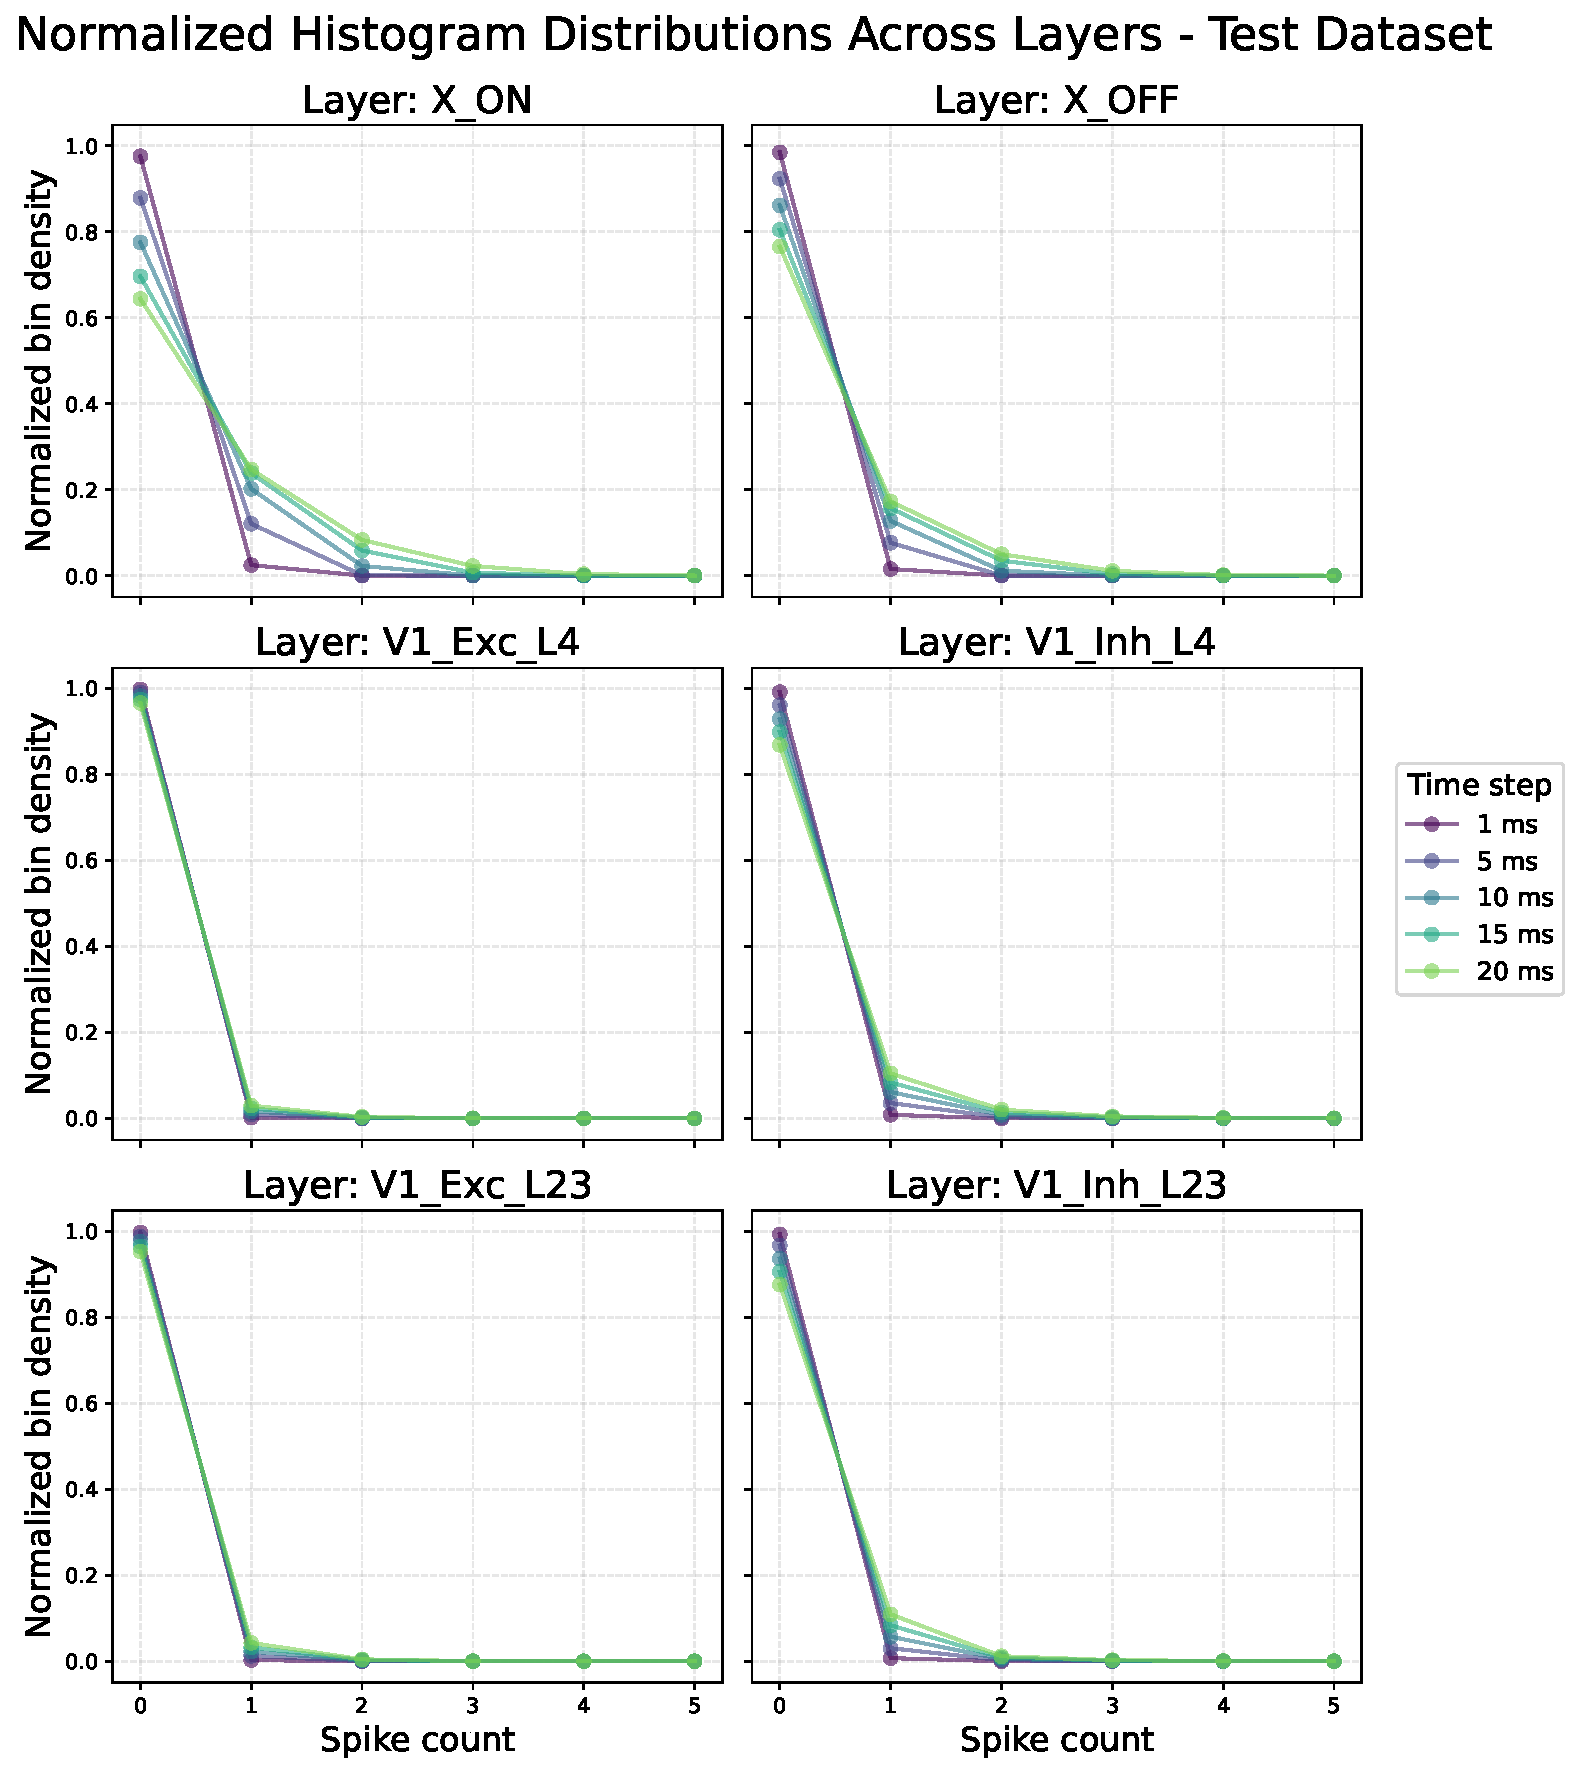
\includegraphics[width=\linewidth]{img/plots/time_step_counts_test.pdf}
    \caption{Evolution of spike counts per time bin with increasing bin size across all neuronal populations in the test dataset.}
    \label{fig:spike_count_distribution_test}
\end{figure}


\subsubsection{Spike Count Distribution Across Time}
\label{subsubsec:spike_time_distribution}
Next, we examine the distribution of spike counts across time for different bin sizes. We propose the following:

\begin{claim}[Temporal Spike Count Distribution]
    The temporal distribution of spike counts per experiment remains consistent across all tested bin sizes. This supports the preservation of temporal response patterns.
\end{claim}

Figures~\ref{fig:temporal_spike_distribution_train} and~\ref{fig:temporal_spike_distribution_test} show the mean spike counts over time for all neuronal populations in the training and test datasets, respectively. These distributions were interpolated to the 1~ms time scale using cubic interpolation.

\begin{figure}
    \centering
    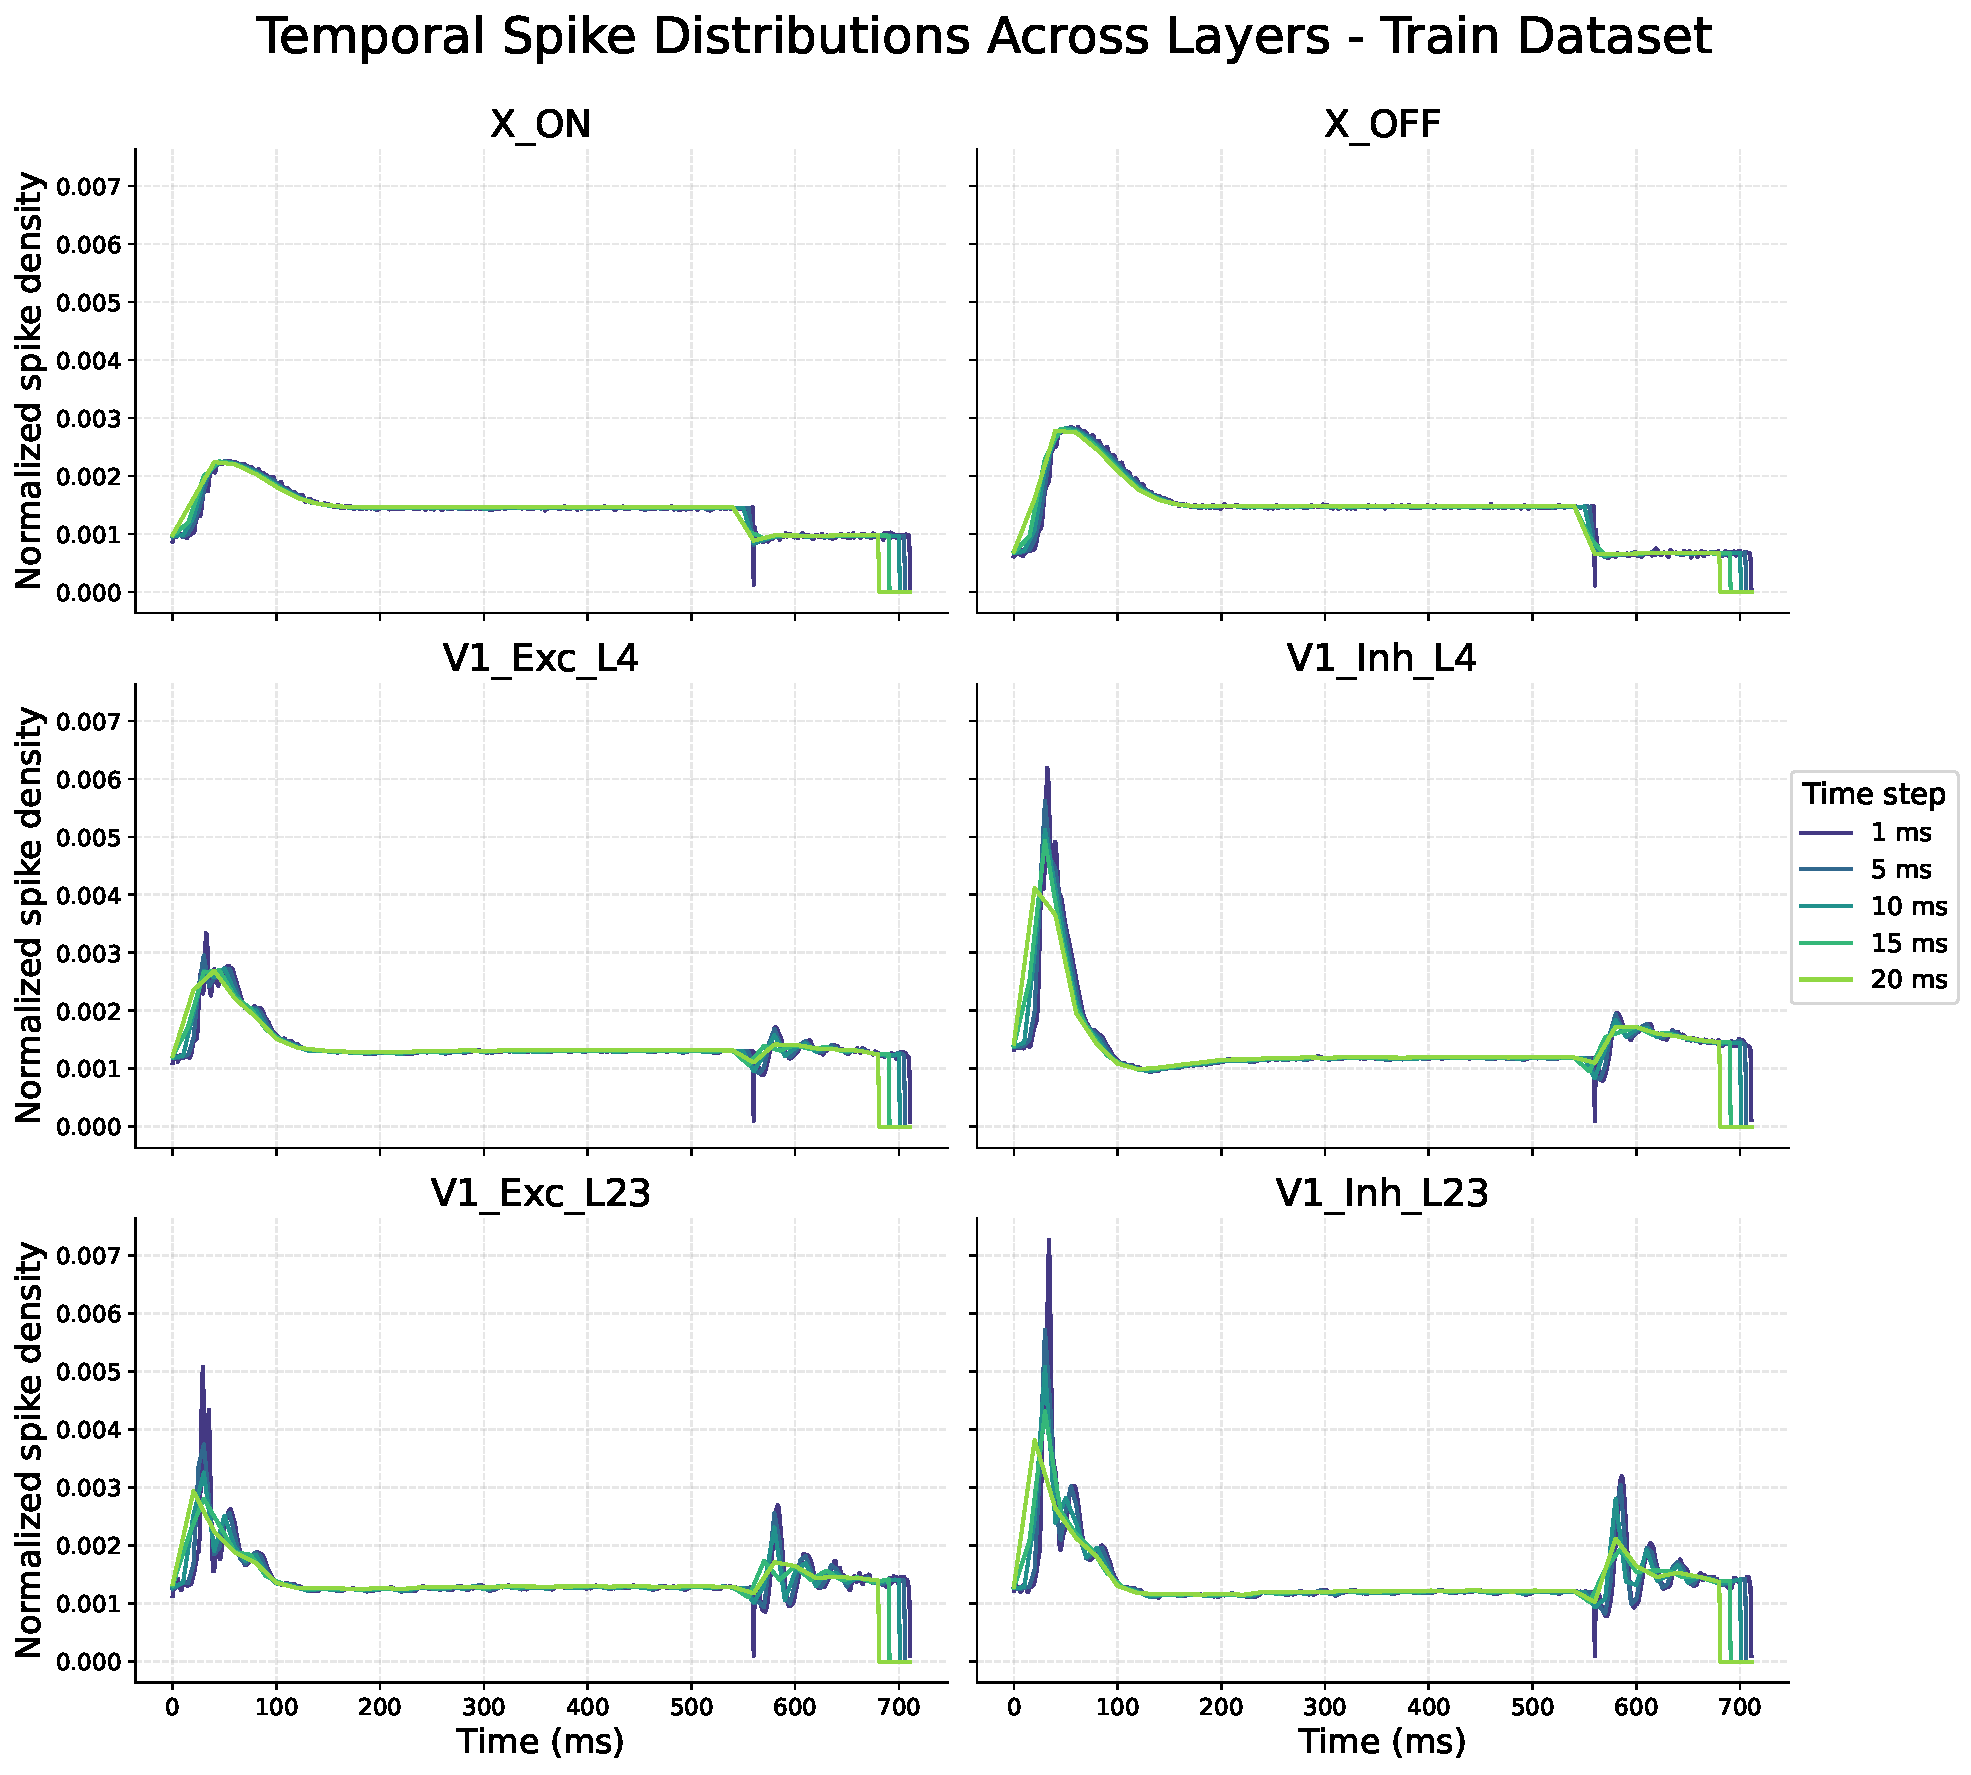
\includegraphics[width=\linewidth]{img/plots/temporal_spike_distribution_train.pdf}
    \caption{Comparison of temporal spike count distributions for different time bin sizes across all neuronal populations in the train dataset. The curves are interpolated to the original 1~ms resolution using cubic interpolation to improve line smoothness.}
    \label{fig:temporal_spike_distribution_train}
\end{figure}

\begin{figure}
    \centering
    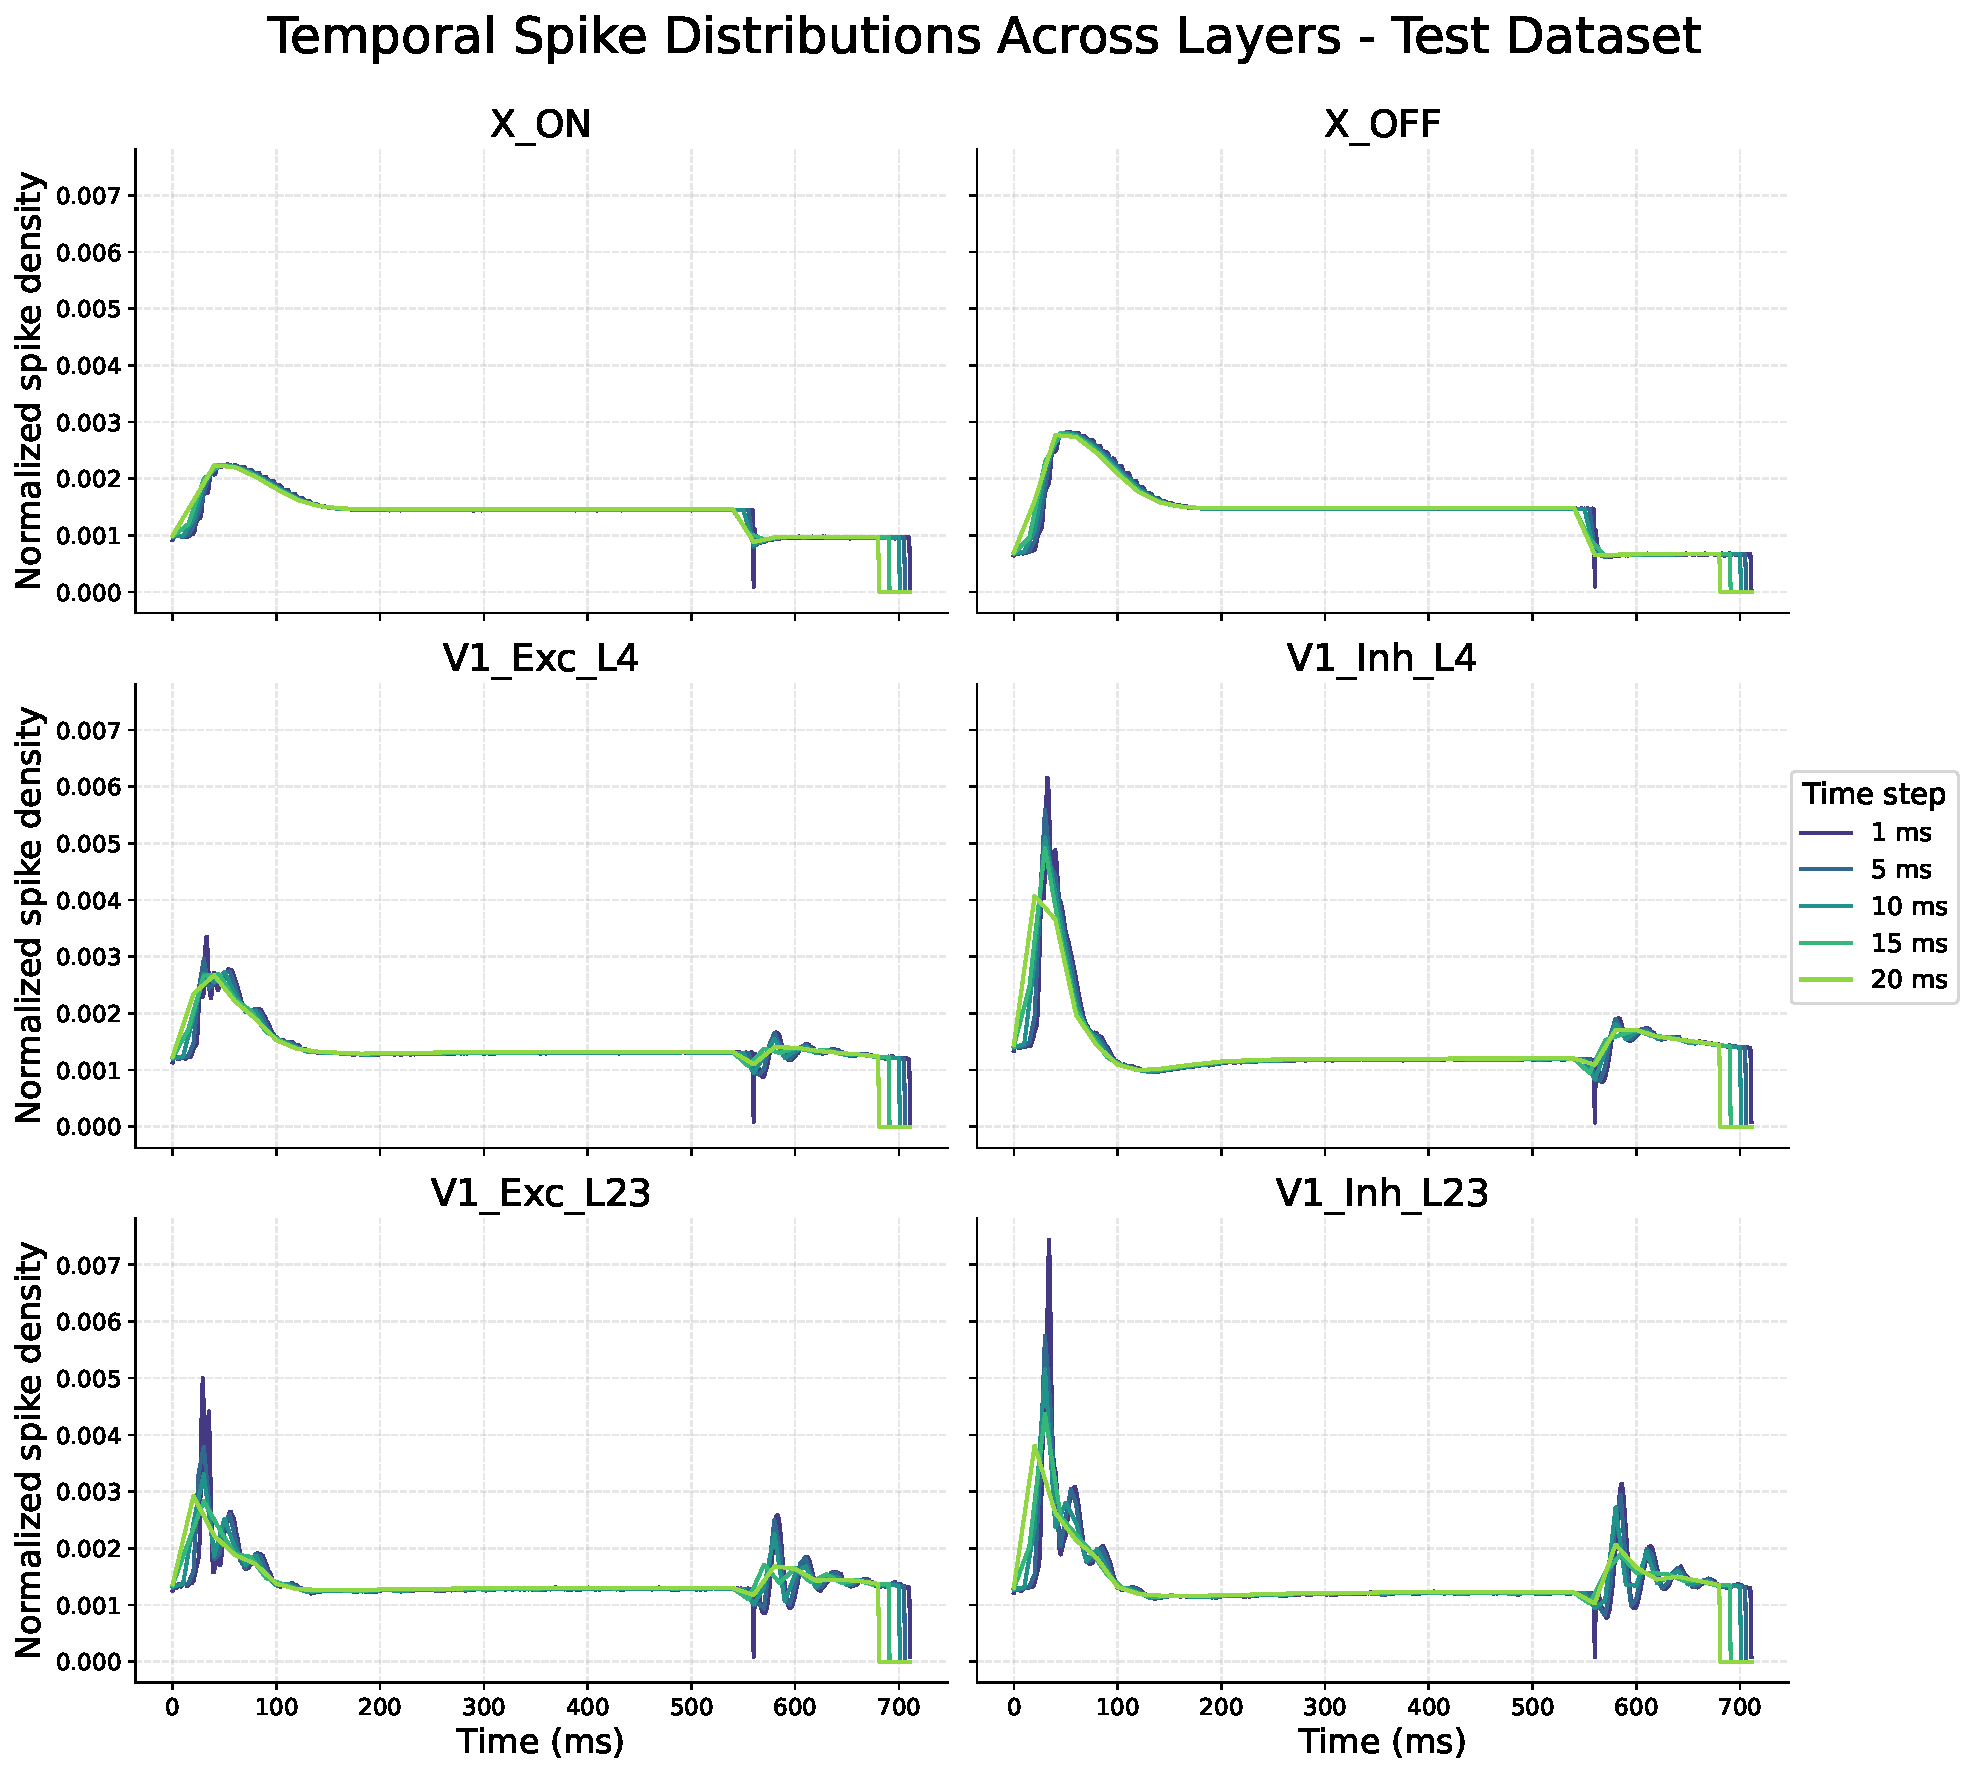
\includegraphics[width=\linewidth]{img/plots/temporal_spike_distribution_test.pdf}
    \caption{Comparison of temporal spike count distributions for different time bin sizes across all neuronal populations in the test dataset. The curves are interpolated to the original 1~ms resolution using cubic interpolation to improve line smoothness.}
    \label{fig:temporal_spike_distribution_test}
\end{figure}

These plots show a clear reduction in noise with increasing bin size, particularly in excitatory layers. The training dataset appears noisier than the test set, likely due to the test set's smaller size and the averaging effect of multiple trials per experiment.

Importantly, the overall distribution shape is preserved across bin sizes. This indicates that binning effectively reduces noise without substantially altering temporal dynamics. Heatmaps in Figure~\ref{fig:correlation_time_bin_size} display Pearson correlation coefficients across different bin sizes, confirming strong similarity in spike distributions over time.

\begin{figure}
    \centering
    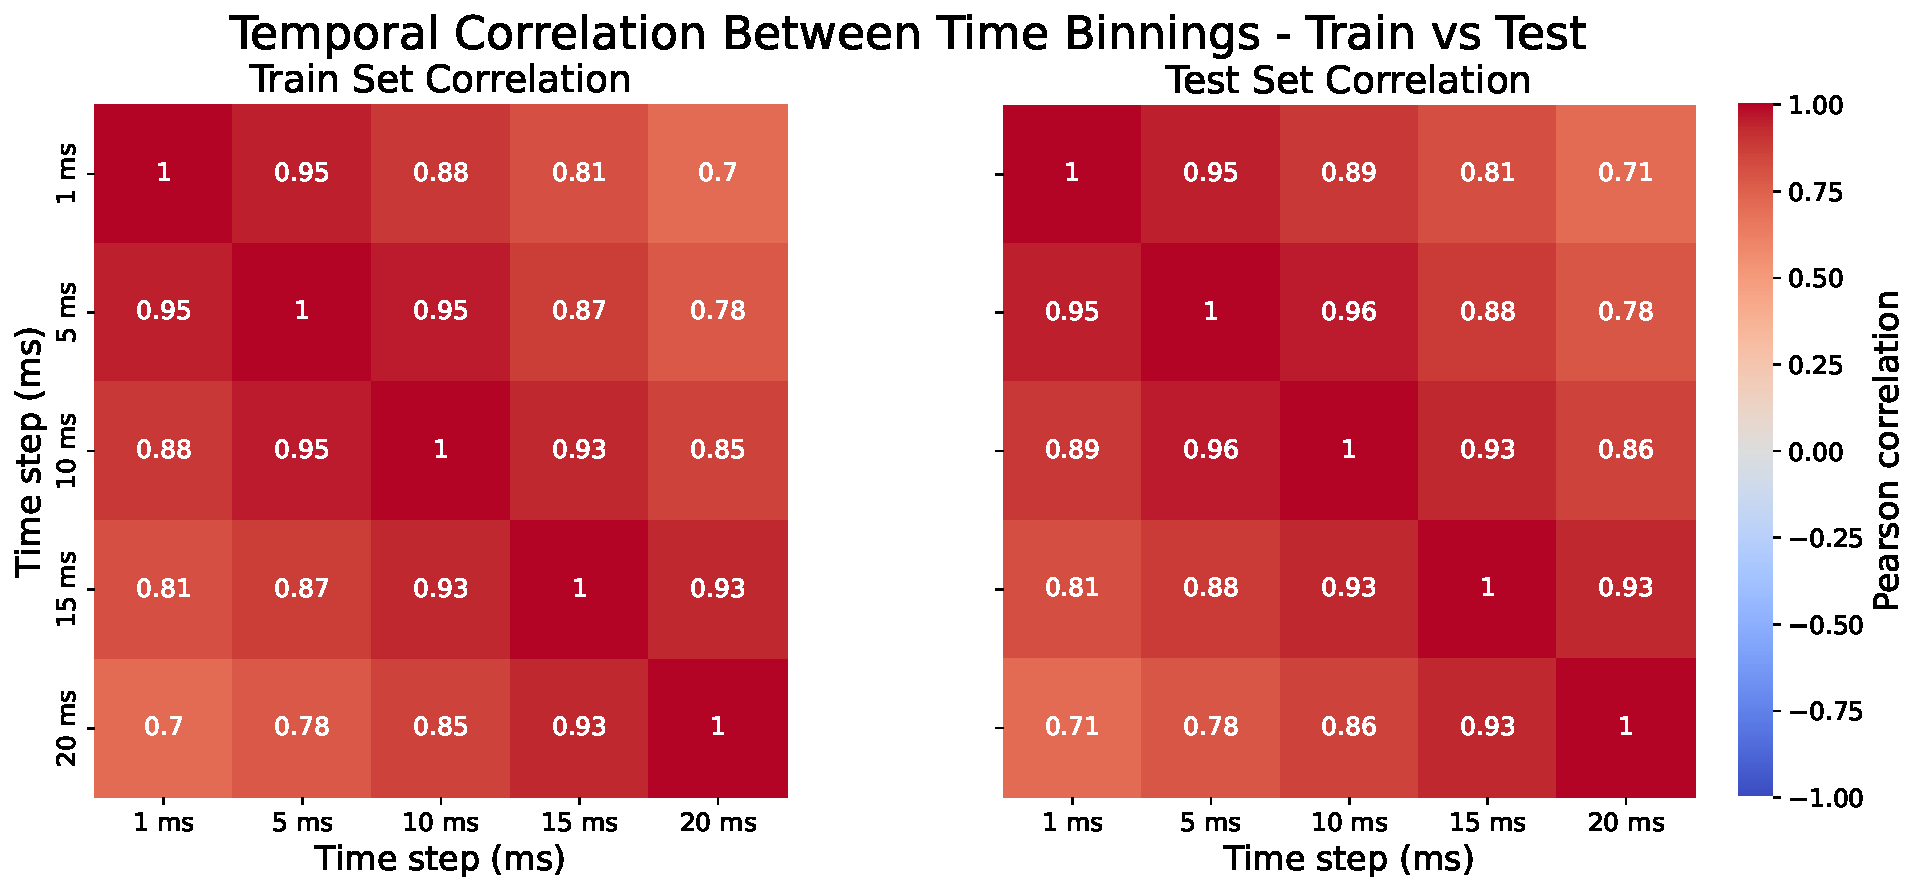
\includegraphics[width=\linewidth]{img/plots/temporal_correlation_time_bin_size.pdf}
    \caption{Heatmaps of Pearson correlation coefficients for spike count distributions over time between different time bin sizes in the train and test datasets.}
    \label{fig:correlation_time_bin_size}
\end{figure}

\subsubsection{Synchrony of Neuronal Populations in Different Time Bins}
\label{subsubsec:neuron_synchrony_binning}

Lastly, we evaluate how time binning affects synchrony, the proportion of neurons firing simultaneously within the same time bin. Synchrony provides insight into the collective temporal dynamics of neuronal populations and is widely studied in neuroscience (\citet{Singer1999}).

Our analysis focuses on the mean synchrony across all time steps. We state the following:

\begin{claim}[Synchrony of Neuronal Populations Across Time Bins]
    The mean synchrony of neuronal populations remains consistent across different time bin sizes. This implies that temporal structure of the dataset is largely preserved.
\end{claim}
\label{claim:synchrony_time_bins_size}

Figures~\ref{fig:boxplot_synchrony_time_train} and~\ref{fig:boxplot_synchrony_time_test} show synchrony distributions for each layer in the training and test datasets. Tables~\ref{tab:synchrony_time_bins_summary_train} and~\ref{tab:synchrony_time_bins_summary_test} summarize the mean and variance of synchrony values.

\begin{figure}
    \centering
    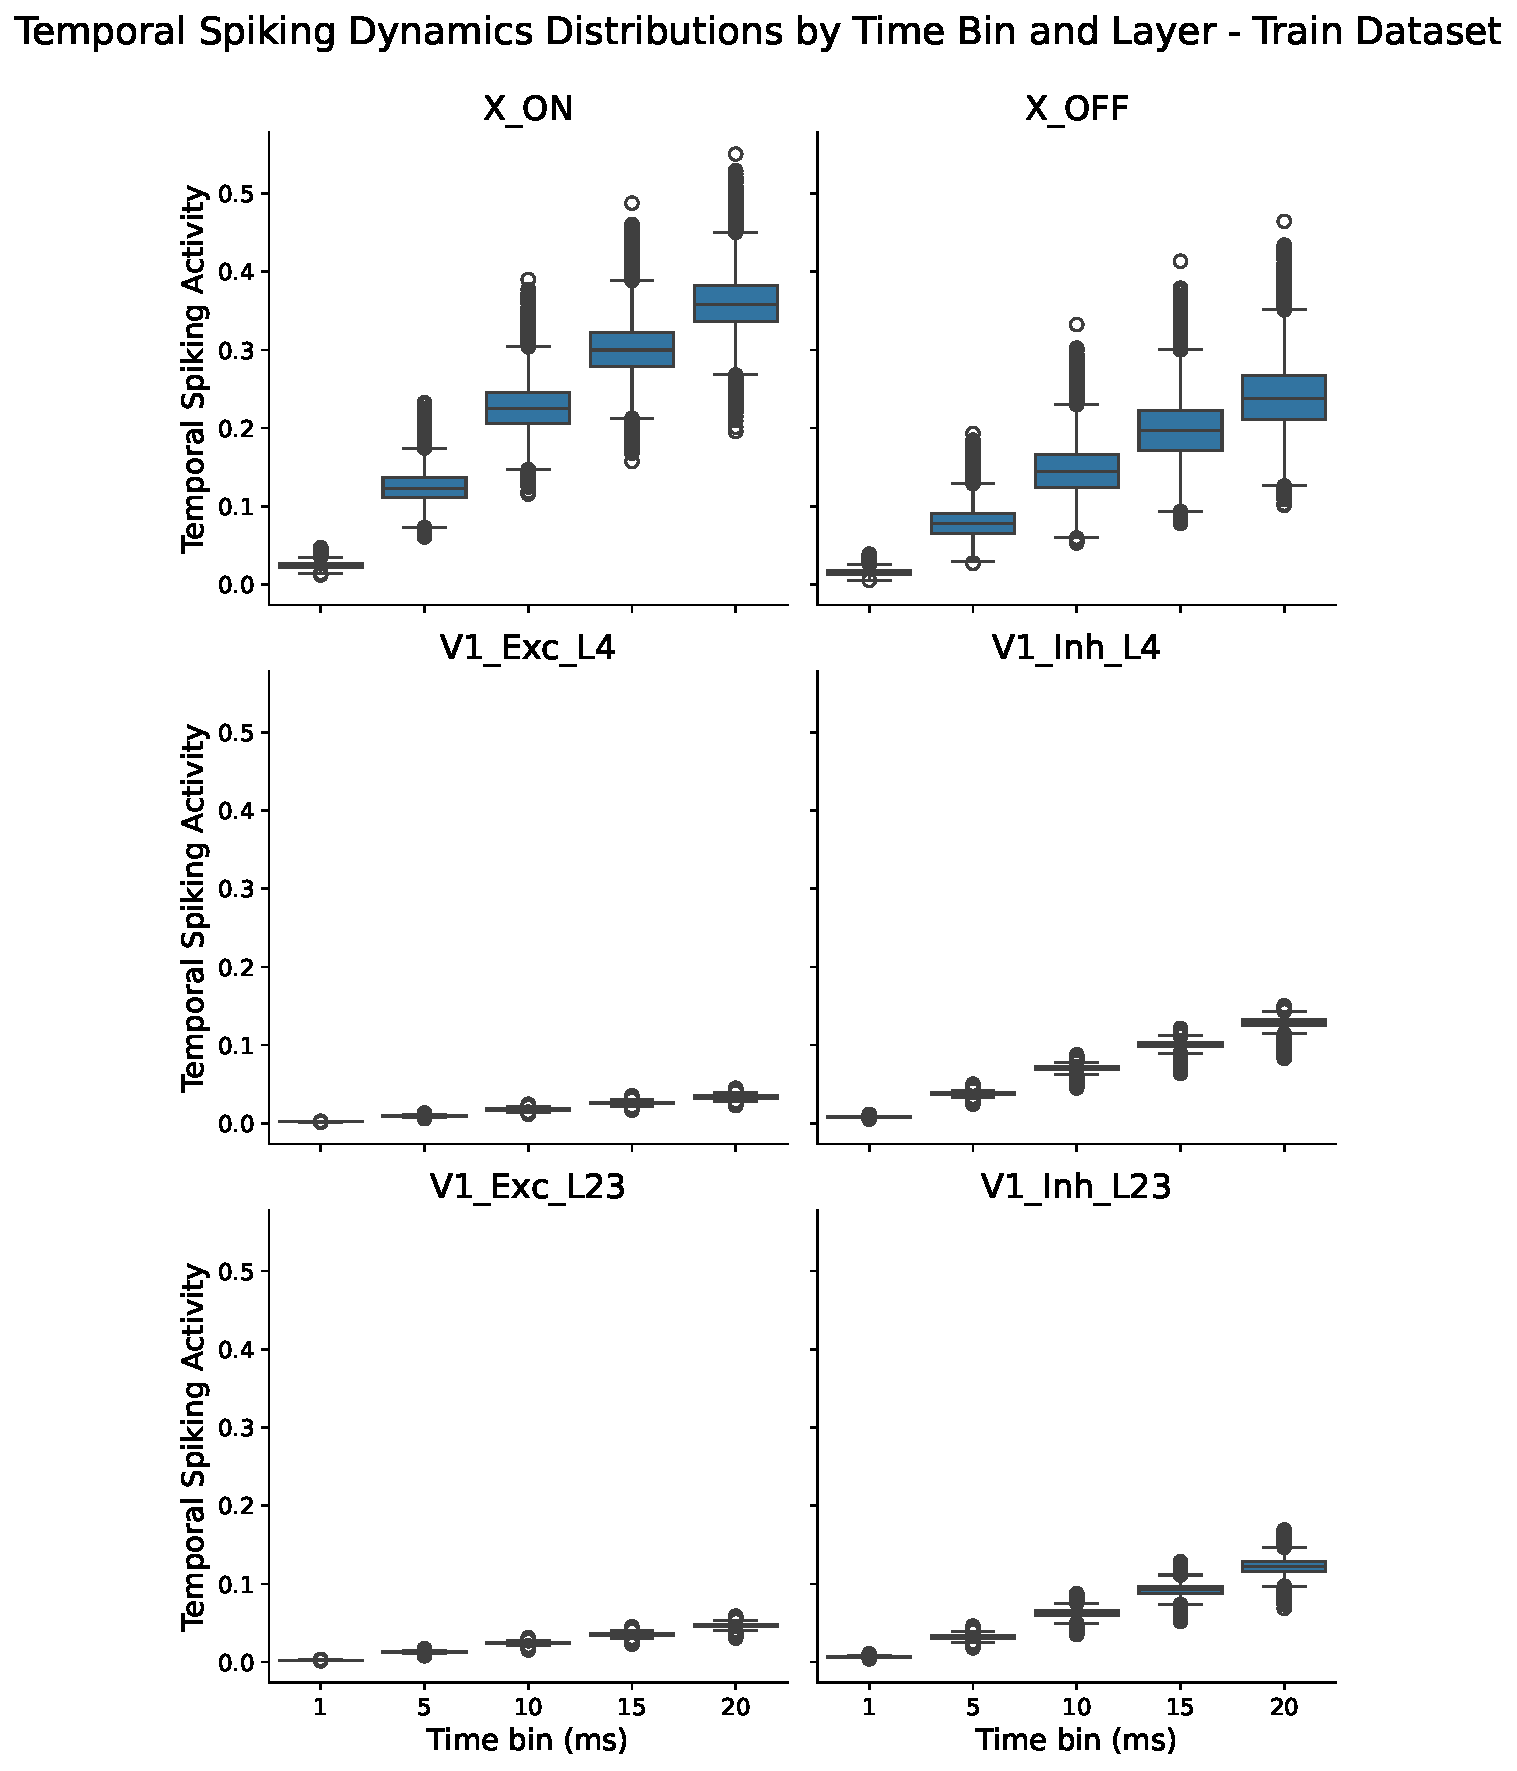
\includegraphics[width=0.92\linewidth]{img/plots/synchrony_boxplot_time_bins_train.pdf}
    \caption{Distribution of mean population synchrony across different time bin sizes for all neuronal populations in the train dataset. The boxplot represents the distribution of mean synchrony values calculated across all experiments}
    \label{fig:boxplot_synchrony_time_train}
\end{figure}


\begin{figure}
    \centering
    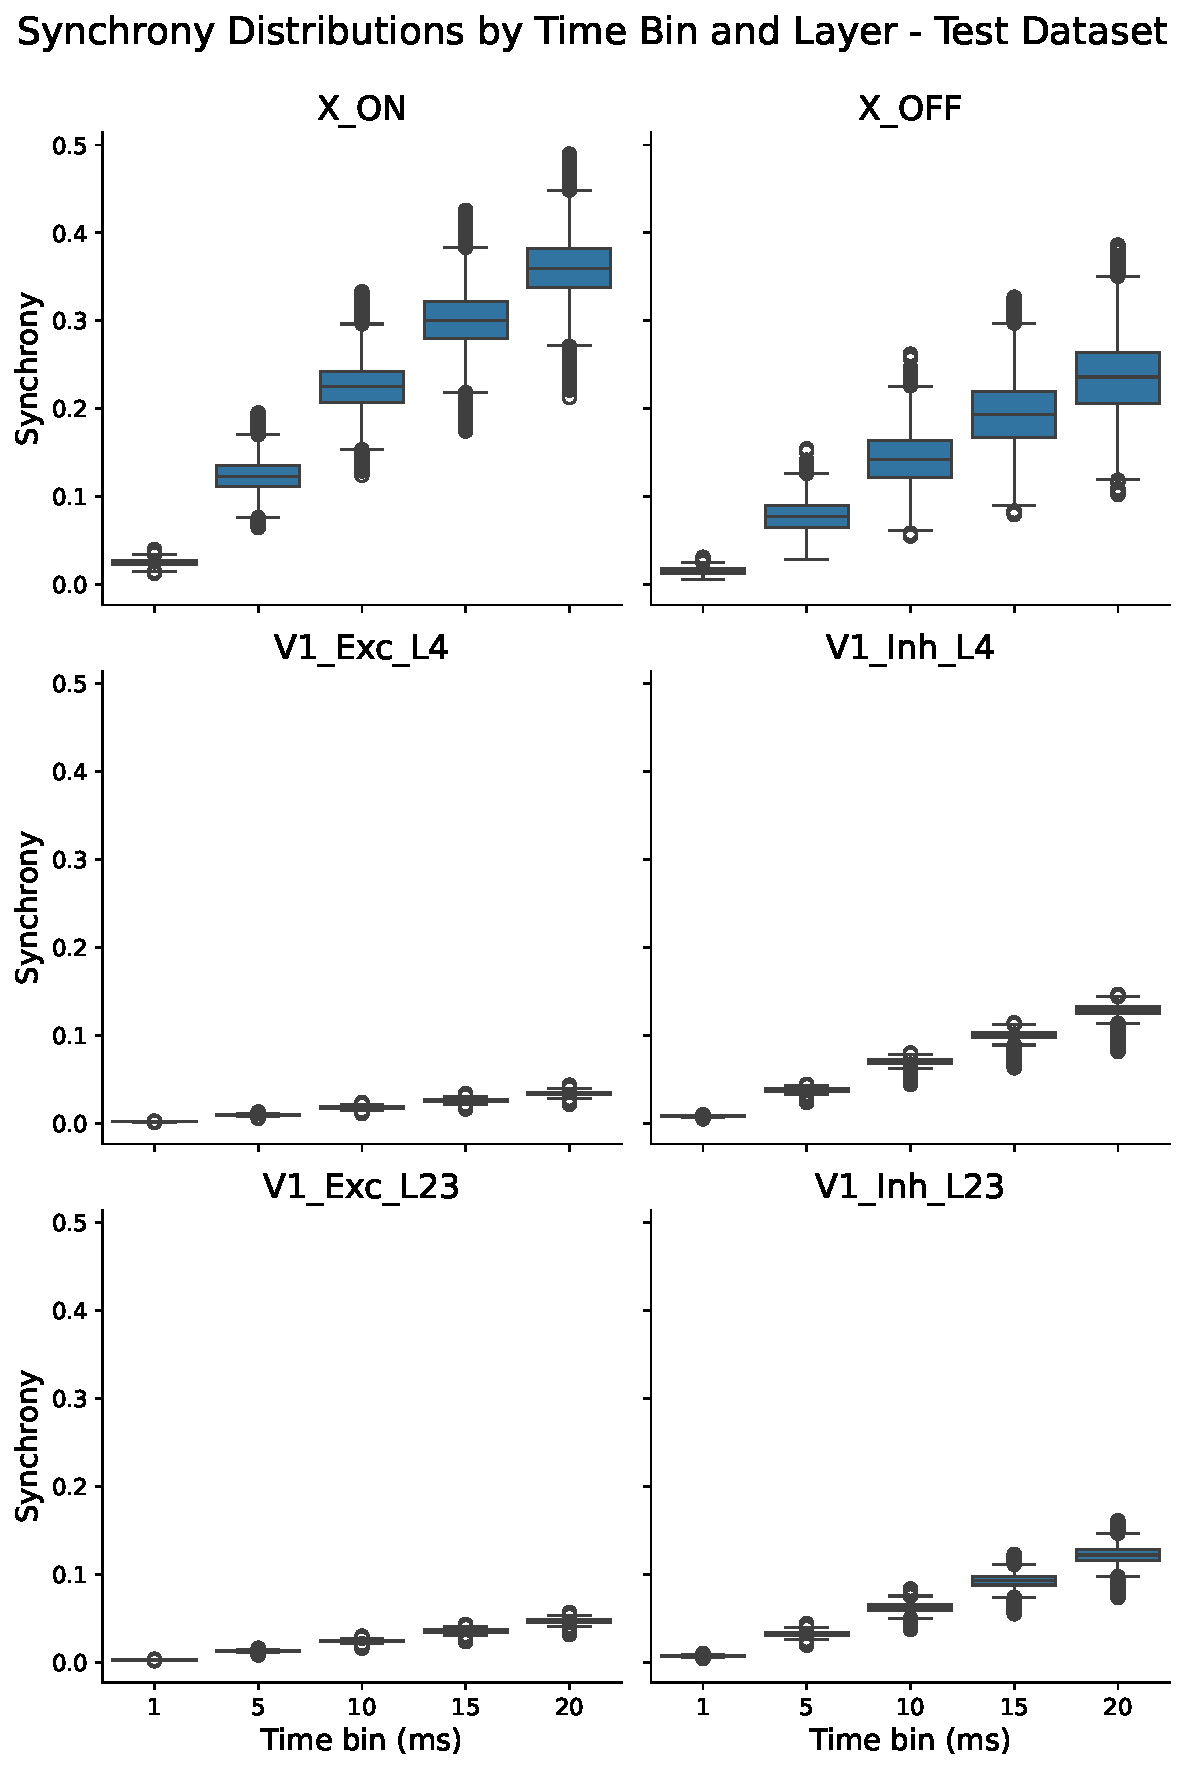
\includegraphics[width=0.92\linewidth]{img/plots/synchrony_boxplot_time_bins_test.pdf}
    \caption{Distribution of mean population synchrony across different time bin sizes for all neuronal populations in the test dataset. The boxplot represents the distribution of mean synchrony values calculated across all experiments}
    \label{fig:boxplot_synchrony_time_test}
\end{figure}

\begin{table}
    \centering\footnotesize\sf
    \begin{tabular}{lrr}
    \toprule
    time step & mean & variance \\
    \midrule
    1 & 0.0101 & 0.0001 \\
    5 & 0.0494 & 0.0018 \\
    10 & 0.0912 & 0.0057 \\
    15 & 0.1256 & 0.0098 \\
    20 & 0.1551 & 0.0134 \\
    \addlinespace % a nice non-intrusive separator of data groups (or final table sums)
    \bottomrule
    \end{tabular}
    \caption{\textbf{Summary of synchrony statistics across time bin sizes in the train dataset:} This table reports the mean and variance of population synchrony across all layers for each time bin size.}
    \label{tab:synchrony_time_bins_summary_train}
\end{table}

\begin{table}
    \centering\footnotesize\sf
    \begin{tabular}{lrr}
    \toprule
    time step & mean & variance \\
    \midrule
    1 & 0.0101 & 0.0001 \\
    5 & 0.0491 & 0.0017 \\
    10 & 0.0908 & 0.0057 \\
    15 & 0.1250 & 0.0097 \\
    20 & 0.1545 & 0.0133 \\
    \addlinespace % a nice non-intrusive separator of data groups (or final table sums)
    \bottomrule
    \end{tabular}
    \caption{\textbf{Summary of synchrony statistics across time bin sizes in the test dataset:} This table reports the mean and variance of population synchrony across all layers for each time bin size.}
    \label{tab:synchrony_time_bins_summary_test}
\end{table}

Synchrony increases with larger time bins, reflecting a higher likelihood of coincident spiking. This effect is most pronounced in LGN layers, especially X\_ON, while V1 excitatory layers show a milder change. These findings suggest that while synchrony is affected by bin size, the overall temporal dynamics are preserved.

We conclude that a bin size of 20~ms strikes a practical balance between maintaining temporal fidelity, minimizing data noise, and ensuring computational efficiency.


\subsection{Model Subset Selection Analysis}
\label{subsec:subset_selection_analysis}

In this section, we analyze the impact of selecting a subset of neurons from the original SNN model. As discussed in Section~\ref{subsubsec:subset_selection}, we selected only 10\% of the neurons due to memory constraints and the computational demands of model training. Our primary interest lies in assessing how this subset selection affects the temporal properties of the dataset, which are central to our research.

All experiments in this section are conducted on the dataset with a 20~ms time bin size (as used in our model) and focus on the training dataset unless stated otherwise. As shown previously in Section~\ref{subsubsec:time_bins_merging}, the results from the training and test datasets are largely consistent.

\subsubsection{Total Spike Counts Across Time Bins}
\label{subsubsec:total_spike_counts_subset}
We begin by analyzing the distribution of spike counts in the time bins for the full dataset and for the subset datasets. Table~\ref{tab:subset_spike_count_distribution} summarizes the mean spike count ratios across all model subsets compared to the full dataset.

\begin{table}
    \centering\footnotesize\sf
    \begin{tabular}{rrrr}
        \toprule
        Spike Count & Full Dataset Ratio & Subsets Mean Ratio & Subsets Standard Deviation \\
        \midrule
        0 & 0.9105 & 0.9102 & 0.0004 \\
        1 & 0.0710 & 0.0712 & 0.0003 \\
        2 & 0.0147 & 0.0148 & 0.0001 \\
        3 & 0.0032 & 0.0032 & 0.0000 \\
        4 & 0.0005 & 0.0005 & 0.0000 \\
        5 & 0.0001 & 0.0001 & 0.0000 \\
        \bottomrule
    \end{tabular}
    \caption{\textbf{Comparison of spike count distributions between full and subset datasets:} This table presents the mean spike count ratios and standard deviations across all model subsets, relative to the full dataset.}
    \label{tab:subset_spike_count_distribution}
\end{table}

The table shows that the differences in spike count distributions between the full and subset datasets are minimal, with low standard deviations. This suggests that randomly selecting a subset of neurons does not significantly impact the overall spike count distribution.

\subsubsection{Spike Count Distribution Across Time}
\label{subsubsec:spike_time_distribution_subset}

Next, we compare the temporal spike count distributions of the subset datasets with that of the full dataset. Figure~\ref{fig:temporal_distribution_subset_vs_full_train} shows the mean temporal behavior across layers for both the full dataset and the average of all subsets. The shaded area represents the standard deviation across subsets.
\begin{figure}
    \centering
    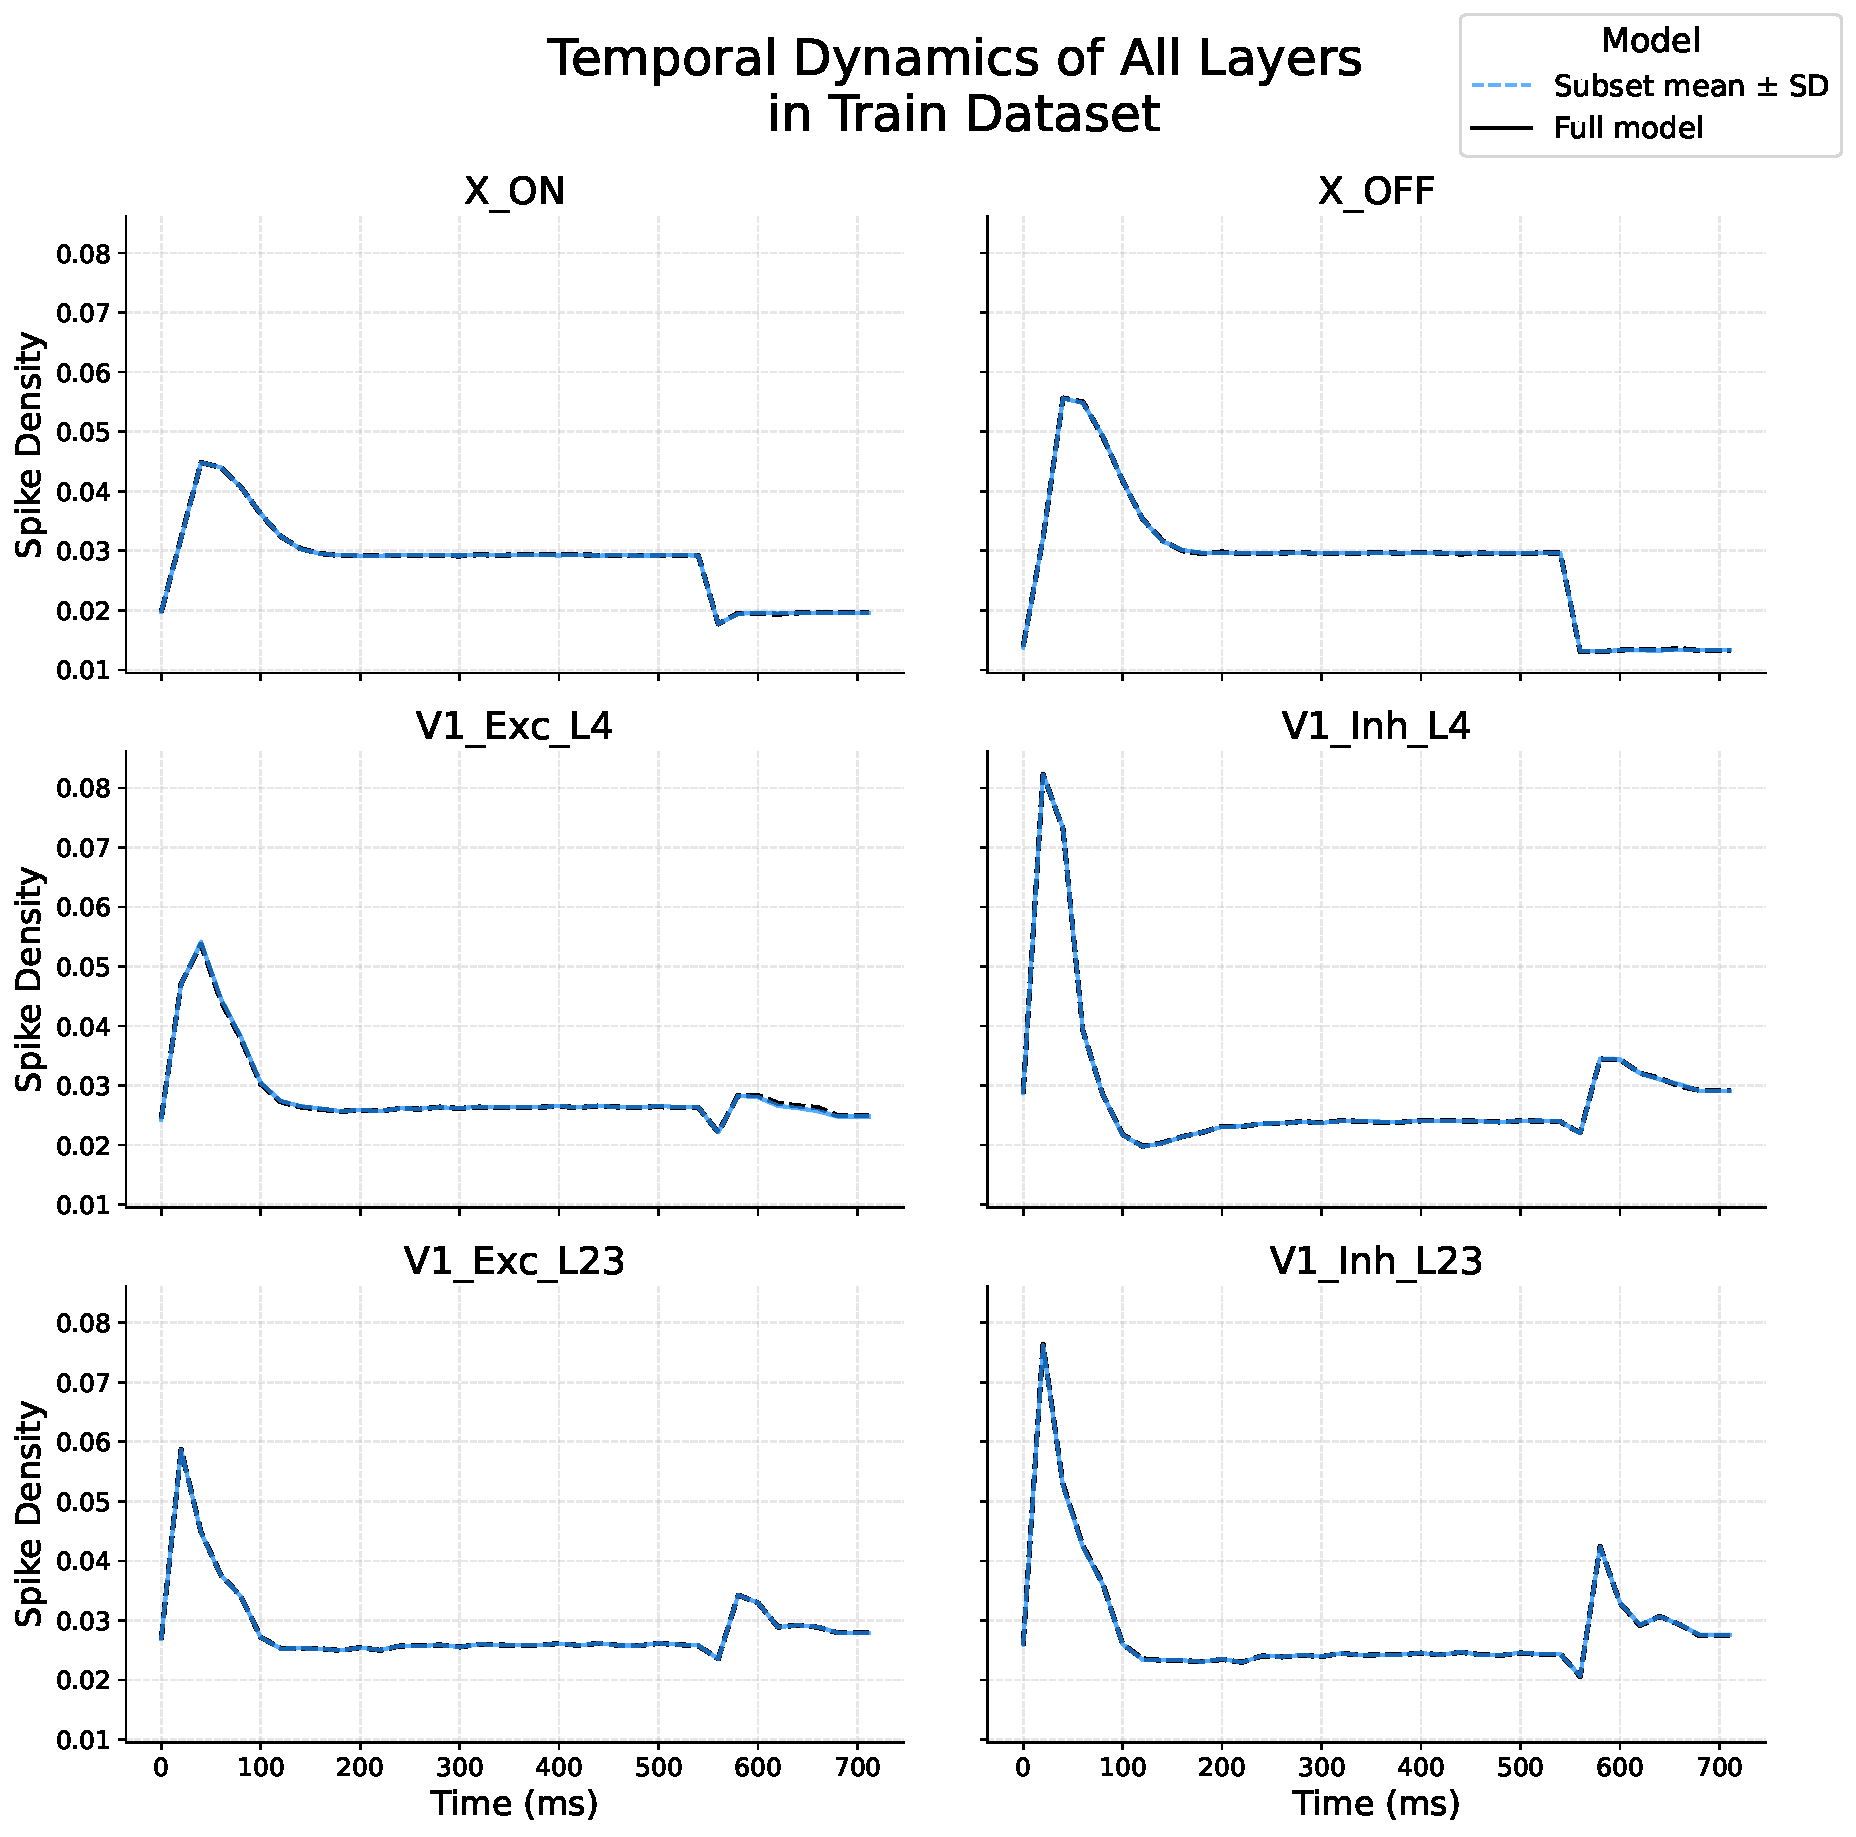
\includegraphics[width=\linewidth]{img/plots/temporal_distribution_subset_vs_full_train.pdf}
    \caption{Comparison of mean temporal activity across layers for the full dataset and the average of all subsets. The shaded area indicates the standard deviation across subsets, which is very small and therefore barely visible in the plot.}
    \label{fig:temporal_distribution_subset_vs_full_train}
\end{figure}

The plot demonstrates that the mean temporal patterns of the subsets closely match those of the full dataset. The small standard deviation further confirms that the temporal properties are preserved despite the neuron subset selection.


\subsubsection{Synchrony of Neuronal Populations in Subsets}
\label{subsubsec:neuron_synchrony_subset}
Finally, we assess the effect of subset selection on neuronal synchrony. Since we are using only a portion of the neurons from the full model, it is possible that groups of neurons that typically spike together may be disrupted, potentially affecting synchrony.

Figure~\ref{fig:boxplot_synchrony_subset} displays a boxplot and jitter plot comparing the synchrony values of the full dataset and all subsets.

\begin{figure}
    \centering
    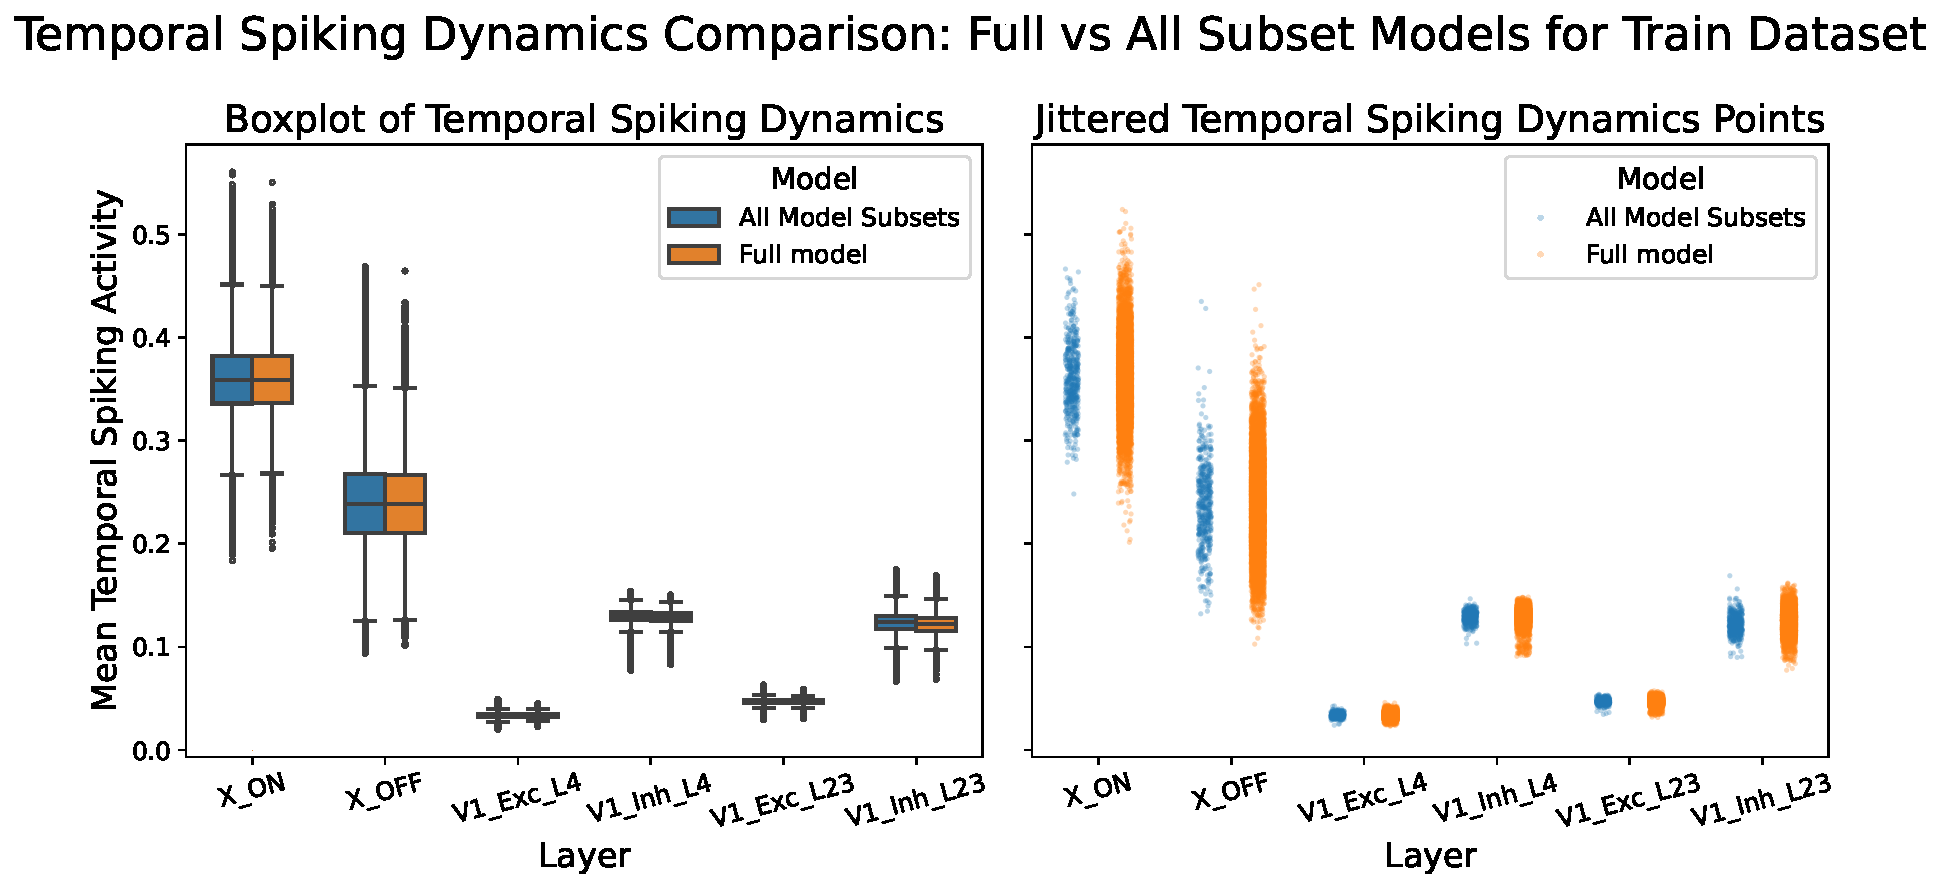
\includegraphics[width=\linewidth]{img/plots/synchrony_comparison_subset_full_train.pdf}
    \caption{Boxplot and jitter plot comparing population synchrony values between the full dataset and all subsets. Each data point represents the mean synchrony of one experiment.}
    \label{fig:boxplot_synchrony_subset}
\end{figure}

As shown, the synchrony distributions are largely similar, particularly in the excitatory layers. This aligns with earlier findings that synchrony variance was low across time bins. Although the jitter plot suggests a slightly narrower spread in the LGN layers for the subsets, the boxplots do not indicate a significant difference.

Based on these observations, we conclude that random selection of 10\% of neurons from the full SNN model does not substantially affect the dataset's statistical or temporal properties. Nevertheless, slight changes in synchrony, particularly in LGN layers, should be taken into account when interpreting model performance results.

\section{Model Evaluation}
\label{sec:model_evaluation}
In this section we focus on the evaluation of the model performance, we compare different model variants and evaluate the influence of each model additional module on the overall results. First, we focus on summary of the results and comparison of all the models based on the high level metrics. Followingly, we focus on the separate inspection of each model perfomance. At the end we focuse on the caveats of our models and try to pin point the aspects of the model that might be the cause of the prediction flaws.

If not stated differently we work with the aggregated values across 20 randomly selected neuronal populations of 10\% size of the original dataset as profoundly described in the Section~\ref{subsubsec:subset_selection}. We have selected 20 randomly chosen subsets to ideally capture the behavior of the model the best without bias caused by the model subset selection.

Throughout this section if not stated differently we will use the uniform naming of the model types that mainly build on the namings defined in the Section~
\ref{sec:model_description}. However, we also compare some model variants with slightly different setup, because of that we need to invent new naming for the differentiation of these throughout the analysis. The naming is the following. We use two simple variant models (Section~\ref{subsec:base_model_architecture}) one with tanh activation function that we note as \emph{simple (tanh)} and the second variant with leakytanh activation function (Section~\ref{subsubsec:leakytanh}) that we note as \emph{simple (leakytanh)}. Then we use only one varian of both \emph{dnn joint} (Section~\ref{subsubsec:dnn_neuron}) and \emph{dnn separate} (Section~\ref{subsubsec:dnn_separate}) for these we keep the naming as it was before. The we use 2 rnn separate (Section~\ref{subsubsec:rnn_neuron_module}) models with different TBPTT time steps that we call \emph{rnn (5 steps)} and \emph{rnn (10 steps)} for either 5 or 10 TBPTT time steps used during the model training. Last model we compare is the model using synaptic depression (Section~\ref{subsubsec:synaptic_depression}) applied only on LGN connections and with 5 TBPTT time steps, this model we label as \emph{syn adapt lgn (5 steps)}. The label part "adapt" comes from the "adaptation", the naming convention for the synaptic depression module used in our model implementation, we kept this naming to facilitate the experimental processing of the data. 

During the evaluation of the model variants on 20 subsets we have used the general setup profoundly described in the Section~\ref{sec:experimental_setup} and additionally for each model variant the hyperparameter setup described in Table~\ref{tab:evaluation_setup}. These hyperparameters has been chosen mainly by the grid search of different experimental setups for each model and partly base on our empirical knowledge and experience throughout the model development. The grid search and selection of the hyperparameters will be deeply descride in the up-comming sections of the chapter.

\begin{table}
    \centering\footnotesize\sf
    \begin{tabular}{lrrrrrrrr}
        \toprule
        Model Variant & Epochs & lr & n-ls & n-nl & n-res & s-ls & s-nl & n-tbptt \\
        \midrule
        simple (tanh) & 10 & 0.000008 & - & - & - & - & - & - \\
        simple (leakytanh) & 10 & 0.000075 & - & - & - & - & - & - \\
        dnn joint & 10 & 0.000010 & 10 & 5 & True & - & - & - \\
        dnn separate & 10 & 0.000010 & 10 & 5 & True & - & - & - \\
        rnn (steps 5) & 40 & 0.000030 & 10 & 3 & True & - & - & 5 \\
        rnn (steps 10) & 40 & 0.000030 & 10 & 3 & True & - & - & 10 \\
        syn adapt lgn (steps 5) & 40 & 0.000030 & 10 & 3 & True & 10 & 2 & 5 \\
        \bottomrule
        \end{tabular}
    \caption{\textbf{Setup of the models in evaluation:} This table presents the setup of each model used in the evaluation results processing. The setup has been mainly selected by the grid search and partially by empirical selection. The columns depicts namely: "Model Variant" - variant of the model, "Epochs" - number of training epochs, "lr" - learning rate, "n-ls" - layer size of the module of neuron, "n-nl" - number of layers of the neuron module, "n-res" - flag whether the neuron module use residual connection, "s-ls" - layer size of the synaptic depression module, "s-nl" - number of layers of synaptic depression module, "n-tbptt" - number of TBPTT time steps. In case the value is not stated (symbol "-"), it is not relevant for the model.}
    \label{tab:evaluation_setup}
\end{table}

\subsection{Overall Model Types Comparison}
\label{subsec:overall_model_types_comparison}
First, we look at the pearson correlation coefficients and normalized cross correlations (Section~\ref{subsec:pearson_cc} and Section~\ref{subsec:normalized_cross_correlation}) comparison of each model performance. The Table~\ref{tab:model_evaluation_overview_comparison} depicts the result overview of every model variant in evaluation and Figure~\ref{fig:model_types_correlation_comparison} shows boxplot comparison of normalized cross correlation and pearson correlation coefficient values across all model subsets.

\begin{table}
    \centering\footnotesize\sf
    \begin{tabular}{lrrrrrrrr}
        \toprule
        Model Variant & N-CC (mean) & P-CC (mean) & N-CC (std) & P-CC (std) \\
        \midrule
        rnn (10 steps) & 0.9212 & 0.7500 & 0.0084 & 0.0082 \\
        rnn (5 steps) & 0.9176 & 0.7471 & 0.0103 & 0.0089 \\
        syn adapt lgn (5 steps) & 0.8935 & 0.7275 & 0.0043 & 0.0042 \\
        dnn joint & 0.8803 & 0.7168 & 0.0021 & 0.0034 \\
        simple (leakytanh) & 0.8778 & 0.7147 & 0.0014 & 0.0032 \\
        dnn separate & 0.8430 & 0.6864 & 0.0940 & 0.0766 \\
        simple (tanh) & 0.2767 & 0.2252 & 0.0400 & 0.0321 \\
        \bottomrule
    \end{tabular}
        
    \caption{\textbf{Summary of Model Performance Metrics:} This table show summary of all model variant normalized cross correlation and pearson correlation coefficients mean and standard deviations across all model subset variants. The results are sorted by the mean normalized cross correlation. The columns depicts namely: "Model Variant" - variant of the model, "N-CC (mean)" - mean of the normalized cross correlation, "P-CC (mean)" - mean of the pearson correlation coefficient, "N-CC (std)" - standard deviation of the normalized cross correlation and "P-CC (std)" - standard deviation of the pearson correlation coefficient.}
    \label{tab:model_evaluation_overview_comparison}
\end{table}

\begin{figure}
    \centering
    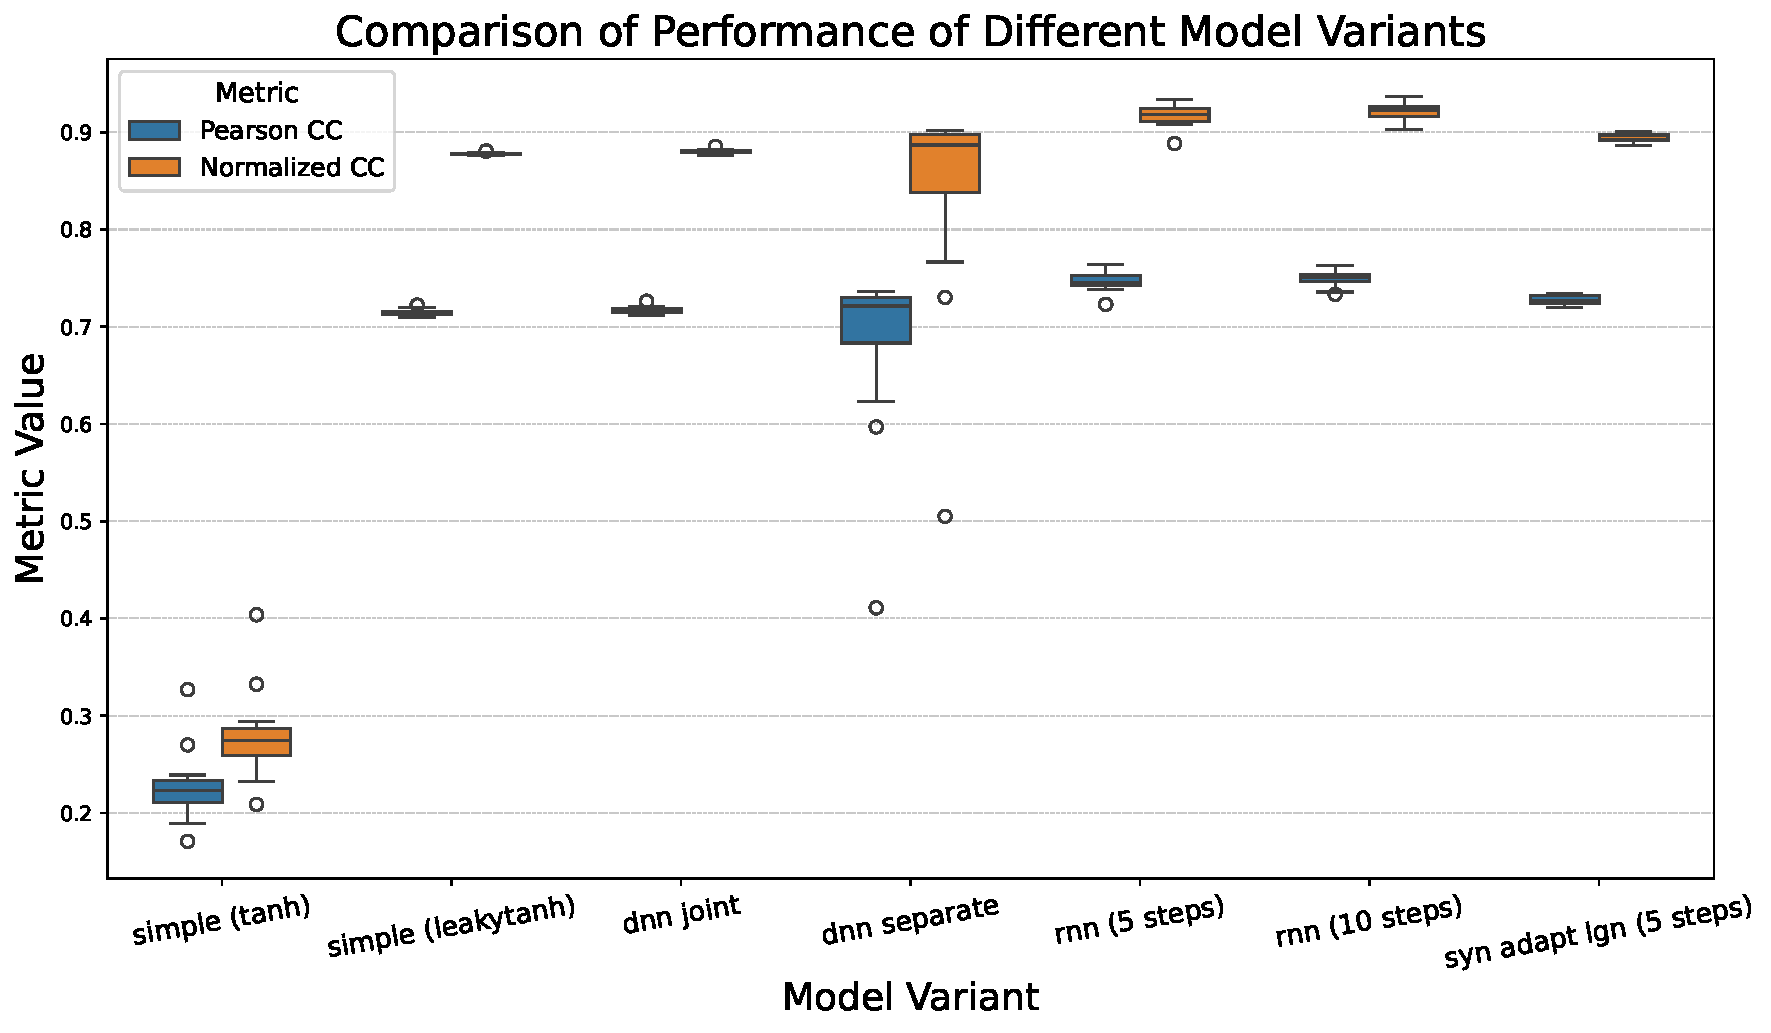
\includegraphics[width=\linewidth]{img/plots/model_types_correlation_comparison.pdf}
    \caption{Boxplot comparing mean Pearson correlation coefficients and normalized correlation coefficients of all model predictions between different model types across all model subsets.}
    \label{fig:model_types_correlation_comparison}
\end{figure}

Overall from the results we can clearly see that the pearson CC and Normalized CC behave fairly similar, only difference is the offset that is expected based on the definition of normalized CC that should be basically pearson CC normalized to smaller range. Building on that we assume from now on that these 2 metrics behave similarly on our data and we will use mainly normalized CC in the rest of our analyses if not stated differently.

From the results we can clearly see that there is one model outstander, the simple (tanh) that clearly performs the worst out of all tested models. On the other hand we can see that using the leakytanh activation function specially designed for the task performs surprisingly well even in the simple model and the model simple leakytanh is even comparable to dnn joint and dnn separate results. This may reflect the fact the the feed-forward dnn neuron modules represent some fairly simple function that we can approximate using some custom activation function like the leakytanh. However, we see that using rnn neuronal module improves our results which may indicate the importance of introducing the memory to our neurons and application of TBPTT training algorithm. 

Another interesting outstander is dnn separate model. This model performs strangely variable in comparison to other model variants. However, we do not really see the clear reason for this behavior. In fact this model should introduce the separation of the excitatory and inhibitory processing in the dnn modules and we expected that it would improve the predictions. Furthermore, while developing the model it showed fairly similar behavior to dnn joint model. For the rnn neuronal modules we have selected only the separate variants since the additional modules should sequentially add more biological plausibility and it really does not sense in our case to omit the layer separation. Also during our empirical tests this model performed fairly similar even sometimes better than the joint variants. We thus suggest that the strange variance might be cause by the not really representative number of results that contains only results for 20 model subset variants and that might be better captured by additional experimental runs on more model subsets. Additionally our testing dataset consists only of 20 trials that might not be enough to compute representative normalized CC values. For the future research it would be definitely worth it to run these experiments on the larger number of subset variants and with larger testing dataset including experiments and trials.

Overall of the models the best performing one seems to be rnn (10 steps) that shows reasonably variability across subset variants and performs best in terms of mean normalized CC. We might also suggest that adding more time steps to TBPTT calculation improves the results. However, experiments on larger number of time steps is not suitable for our experiments for time and memory consumption reasons and our restrained capability to access these.

The last interesting notice from the results is that it seems that the model syn adapt lgn (5 steps) performs worse than the models without synaptic depression module at all. We are not sure about the reason for this phenomenon but it might well be cause by the non-profound grid search for synaptic depression models as well with the necessity for usage of more TBPTT time steps and training epochs. These things unfortunately could not be tested due the computational demands of the synaptic depression models.

\begin{figure}
    \centering
    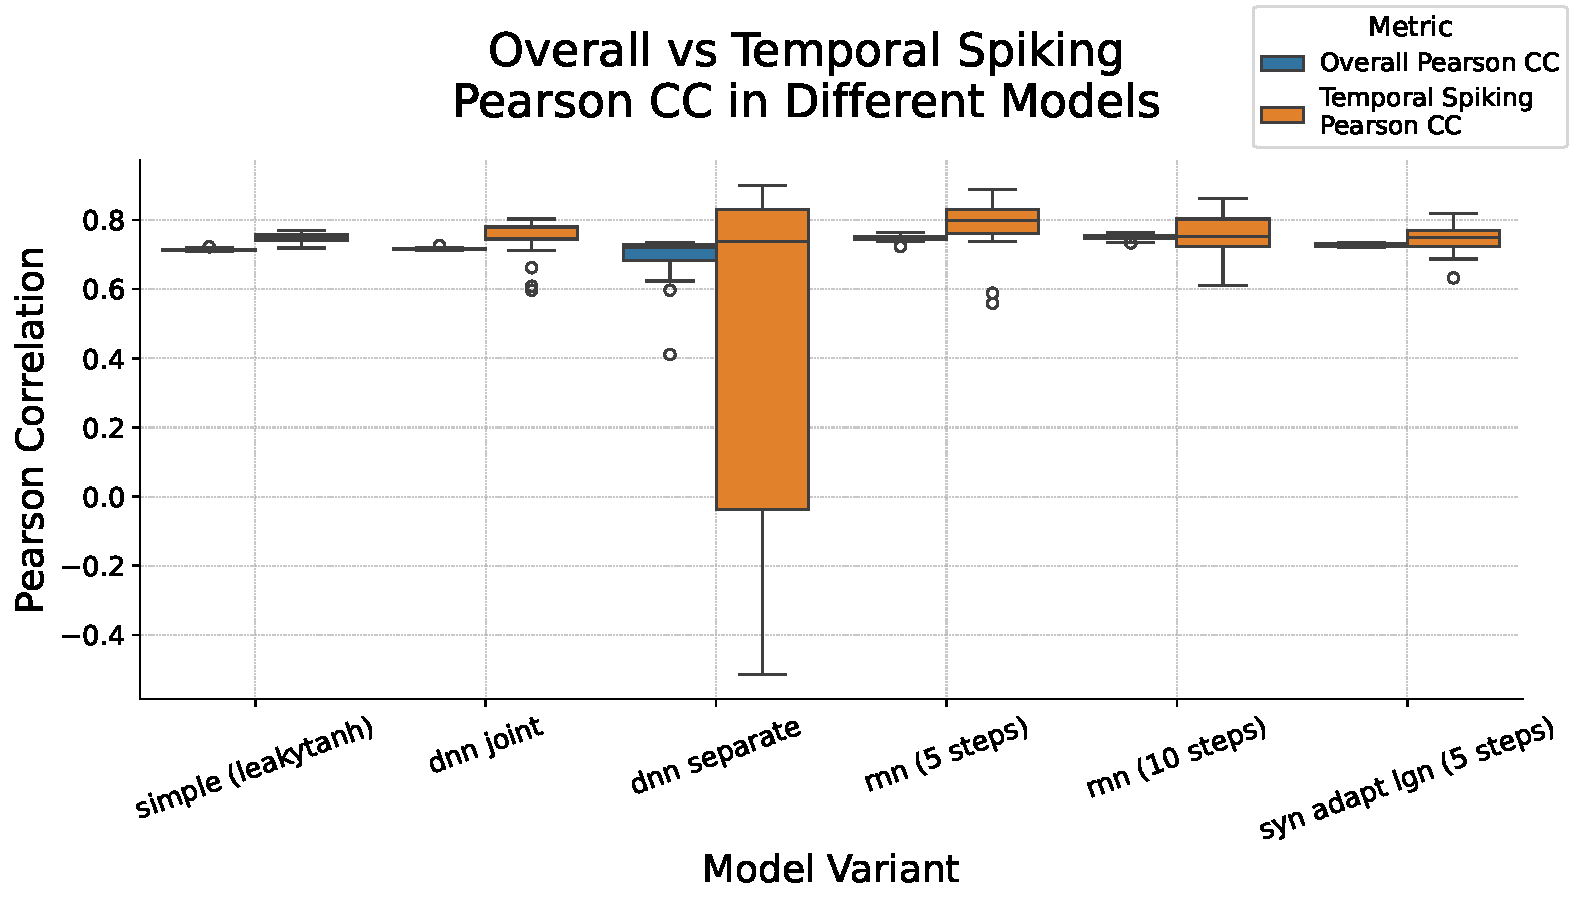
\includegraphics[width=\linewidth]{img/plots/boxplot_model_comparison_synchrony_overall_pearson.pdf}
    \caption{This figure shows comparison of distribution of pearson CC between model predictions and of model prediction synchrony curves across all layers and all model subset variants for each model type in respect targets.}
    \label{fig:boxplot_models_overall_synchrony_pearson_comparison}
\end{figure}


\begin{figure}
    \centering
    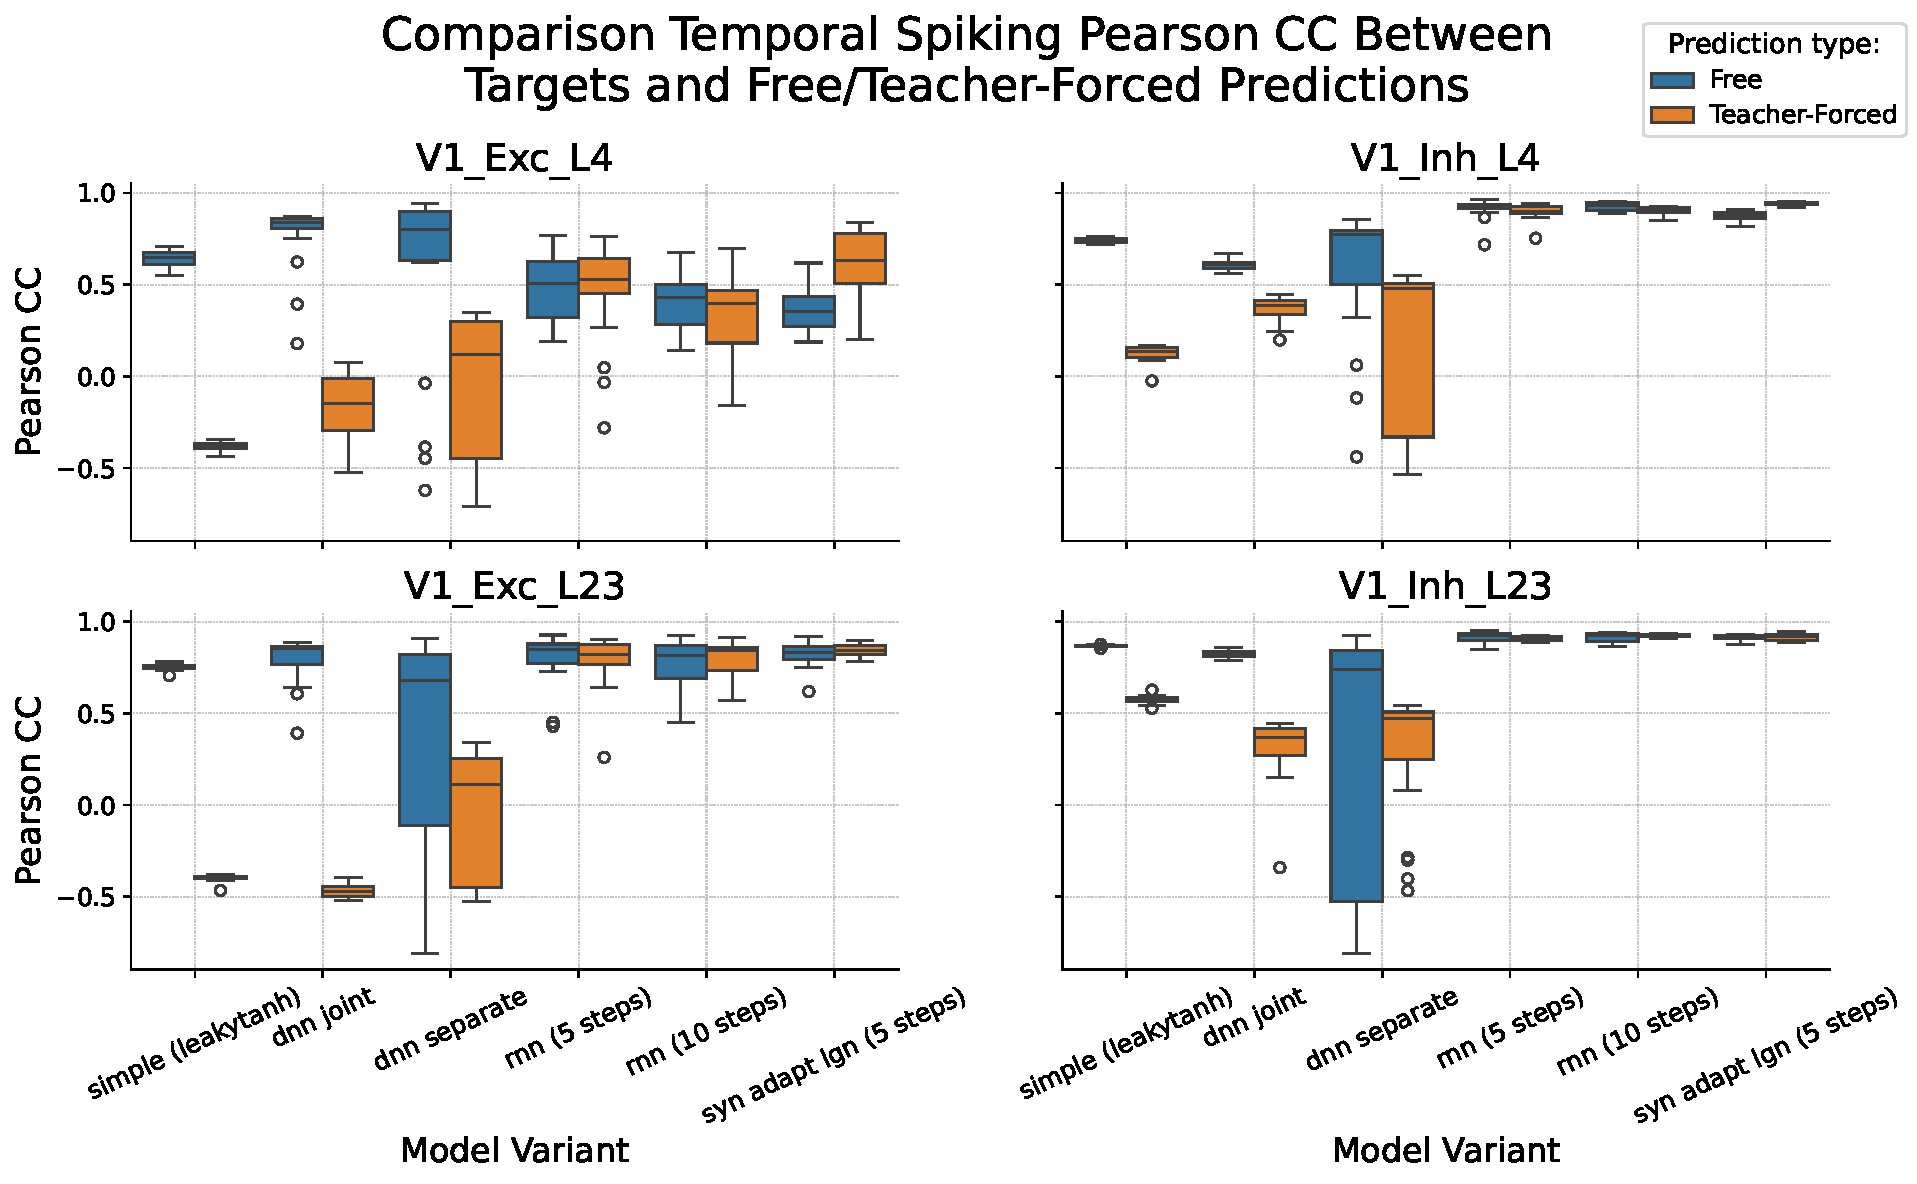
\includegraphics[width=\linewidth]{img/plots/boxplot_model_comparison_synchrony_pearson_layers.pdf}
    \caption{This figure shows comparison of distribution of pearson CC between model prediction and target synchrony curves separately for each layer.}
    \label{fig:boxplot_models_pearson_synchrony_different_layers}
\end{figure}

To empower our claims we have decided to conduct pairwise one-sided Mann-Whitney U test (\citet{mann_whithey_1947}) to test whether the distribution of normalized CC from one model are greater or equal to the normalized CC of the other model. We have selected this test because we do not know from which distribution our sampled normalized CC come from, so, we cannot really use some stronger more powerful parametric test. This test tests hypothesis that the two sampled groups are taken from the same distribution. Since we are using the one-sided variant we test the hypothesis that one sample is sampled from the distribution that is greater or equal to the other population. We have visualized the p-values of each tested pair in the heatmap depicted in the Figure~\ref{fig:model_types_p_values_heatmap}. In this heatmap the model in the row symbolizes the model that performs better in terms of the normalized CC in comparison to model in the row.

\begin{figure}
    \centering
    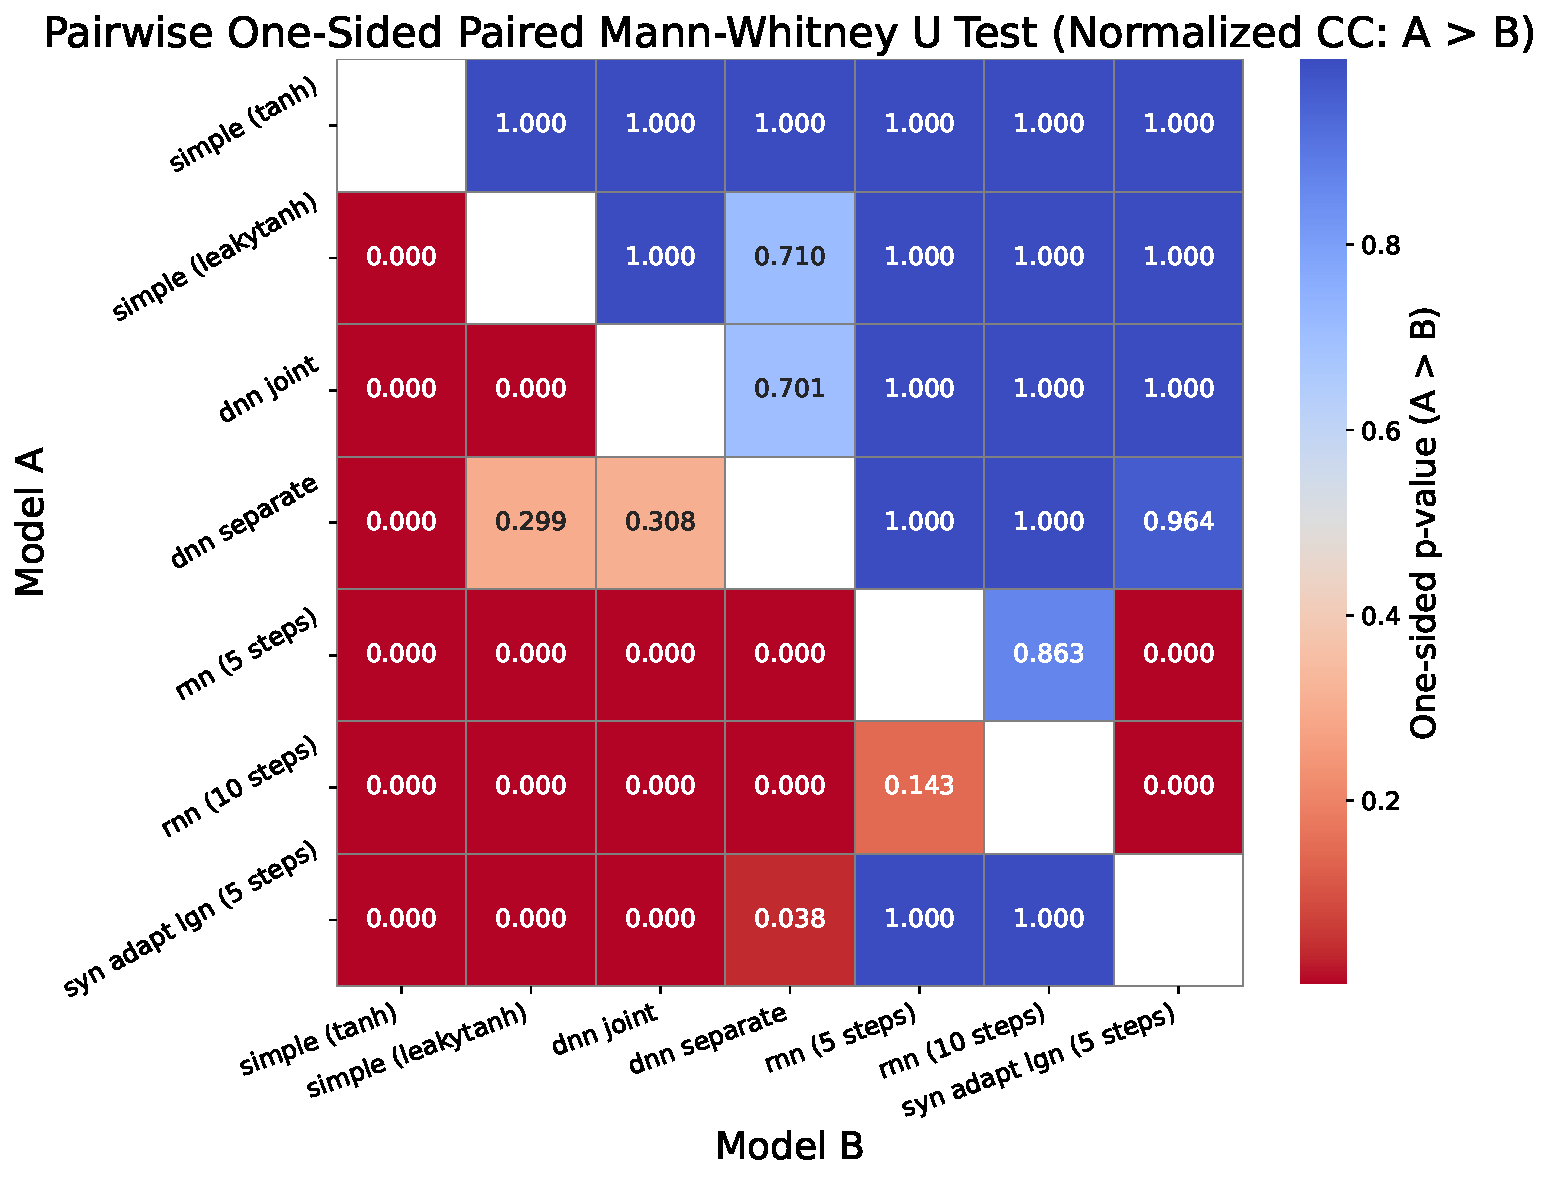
\includegraphics[width=\linewidth]{img/plots/model_types_p_value_heatmap_cc_norm.pdf}
    \caption{Heatmap that shows the p-value of pairwise one-sided Mann-Whitney U test. The test has been performed on the values of normalized cross correlation of each subset of each model variant. The test should say whether one of the model has significantly higher normalized cross correlation values. In each tile the row value marked as "Model A" represents the model that is tested to perform better and column value marked as "Model B" represents the model that is tested to perform worse. Assuming significance level $\alpha=0.05$ the value smaller than $\alpha$ decline the null hypothesis that the normalized cross correlation distribution is the same or worse for "Model A".}
    \label{fig:model_types_p_values_heatmap}
\end{figure}

The tests mainly confirms our claims that we have concluded from the box plots and the mean and standard deviation. If we assume the significance level $\alpha=0.05$ then we decline the hypotheses that simple (tanh) performs better than arbitrary other model variant. While looking at the other variants it mostly seems that the more complex models perform better with two exceptions. The dnn separate model that behaved strangely mainly in terms of the large variance that we already mentioned and the syn adapt lgn (5 steps) that interestingly seems to perform worse than the rnn model variants without the synaptic depression modules. This fact may be caused by the several constraints already mentioned before connected to constrained computational resources and thus not that profound analysis of the hyperparameters. Additionally, we have not tested the synaptic depression variant that applies the synaptic depression module to all connections since its computational complexity.

Overall, based on the high level metrics of person CC and normalized CC we assume that majority of our additional modules improved our model performance and that additional biological constraints might lead to improved modeling of the neural responses. The only two exceptions that seemingly contradicts this statement are dnn separate model and syn adapt lgn (step 5) model. These facts we mainly assign to our limited ability to test the model performances deeply and thus our results might not cover all model properties comprehensively.

\subsection{Prediction-Target Comparison of Model Variants}
\label{subsec:prediction_target_comparison_variants}


\subsubsection{Simple Model With LeakyTanh Activation}
\label{{subsubsec:simpl_leakytanh_eval}}
\begin{figure}
    \centering
    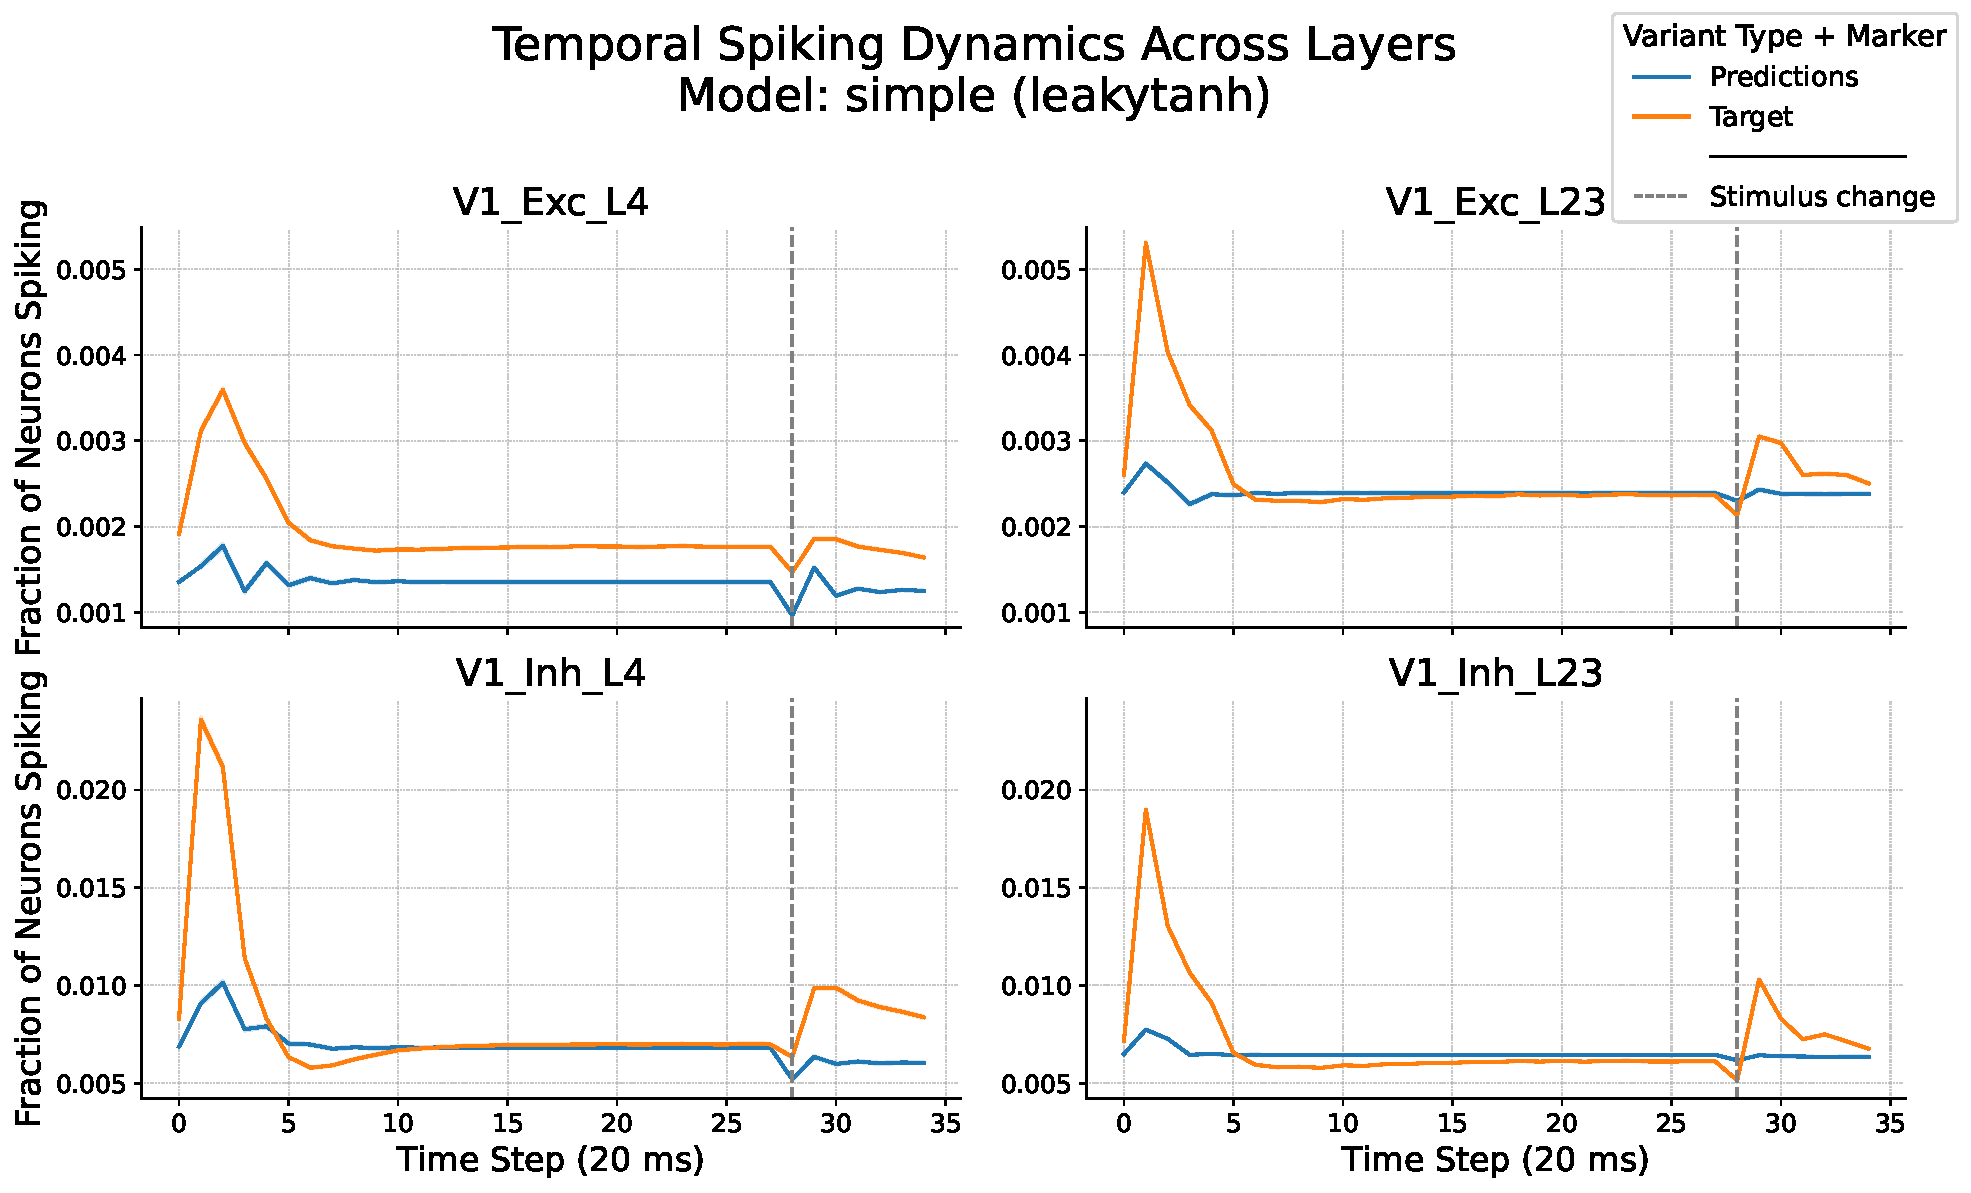
\includegraphics[width=\linewidth]{img/plots/separate_model_synchrony_curve_simple_evaluation_new.pdf}
    \caption{This figure depicts mean synchrony curve of simple (leakytanh) model predictions and its comparison to mean target synchrony curve both across all trials and all model subset variants including error bars. The dashed line marks the time step where the natural stimuli and blank stimuli changes.}
    \label{fig:synchrony_curve_simple_leaky_tanh}
\end{figure}

\subsubsection{DNN Joint Model}
\label{{subsubsec:dnn_joint_eval}}

\begin{figure}
    \centering
    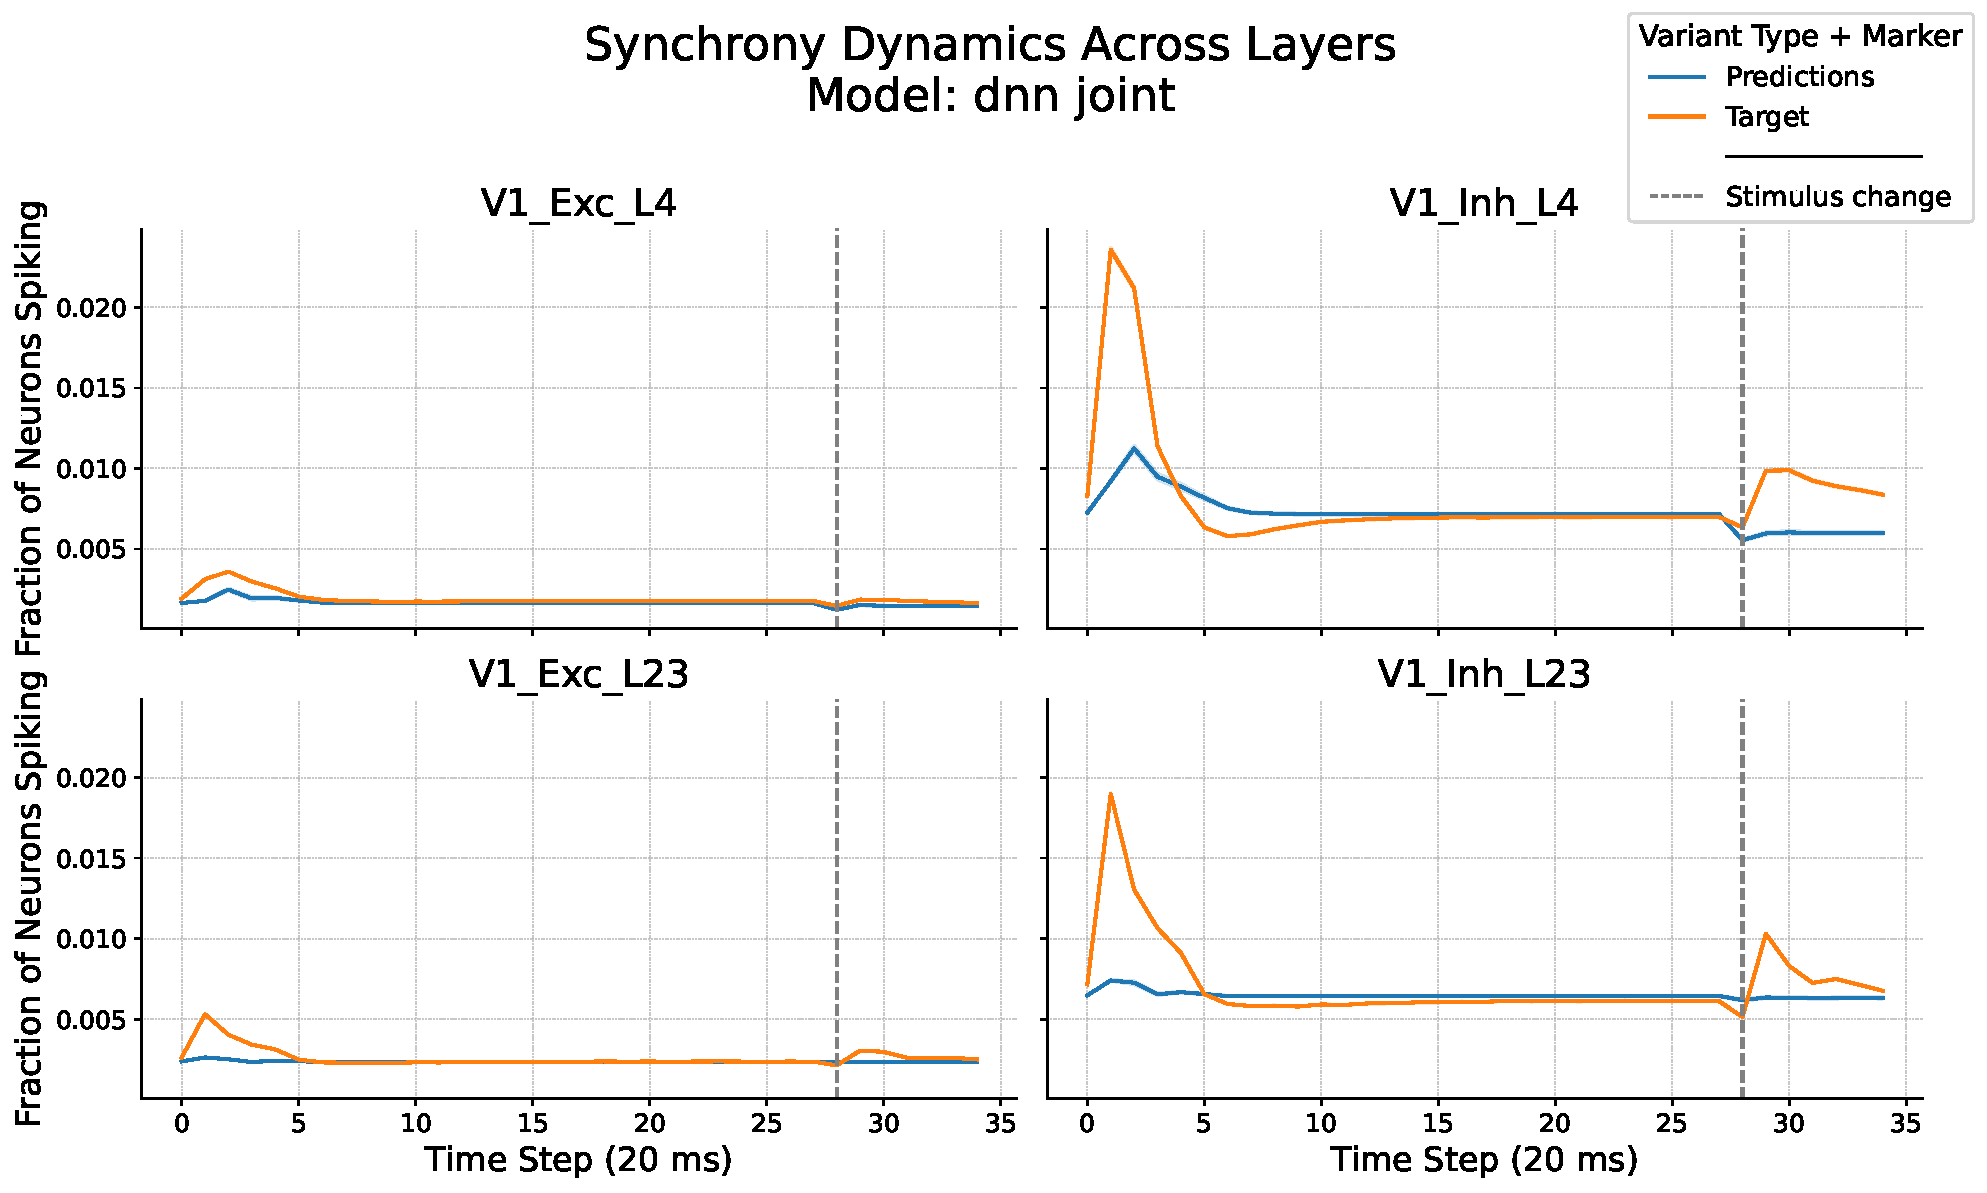
\includegraphics[width=\linewidth]{img/plots/separate_model_synchrony_curve_dnn_joint_evaluation.pdf}
    \caption{This figure depicts mean synchrony curve of dnn joint model predictions and its comparison to mean target synchrony curve both across all trials and all model subset variants including error bars. The dashed line marks the time step where the natural stimuli and blank stimuli changes.}
    \label{fig:synchrony_curve_dnn_joint}
\end{figure}


\subsubsection{DNN Separate Model}
\label{{subsubsec:dnn_separate_eval}}
\begin{figure}
    \centering
    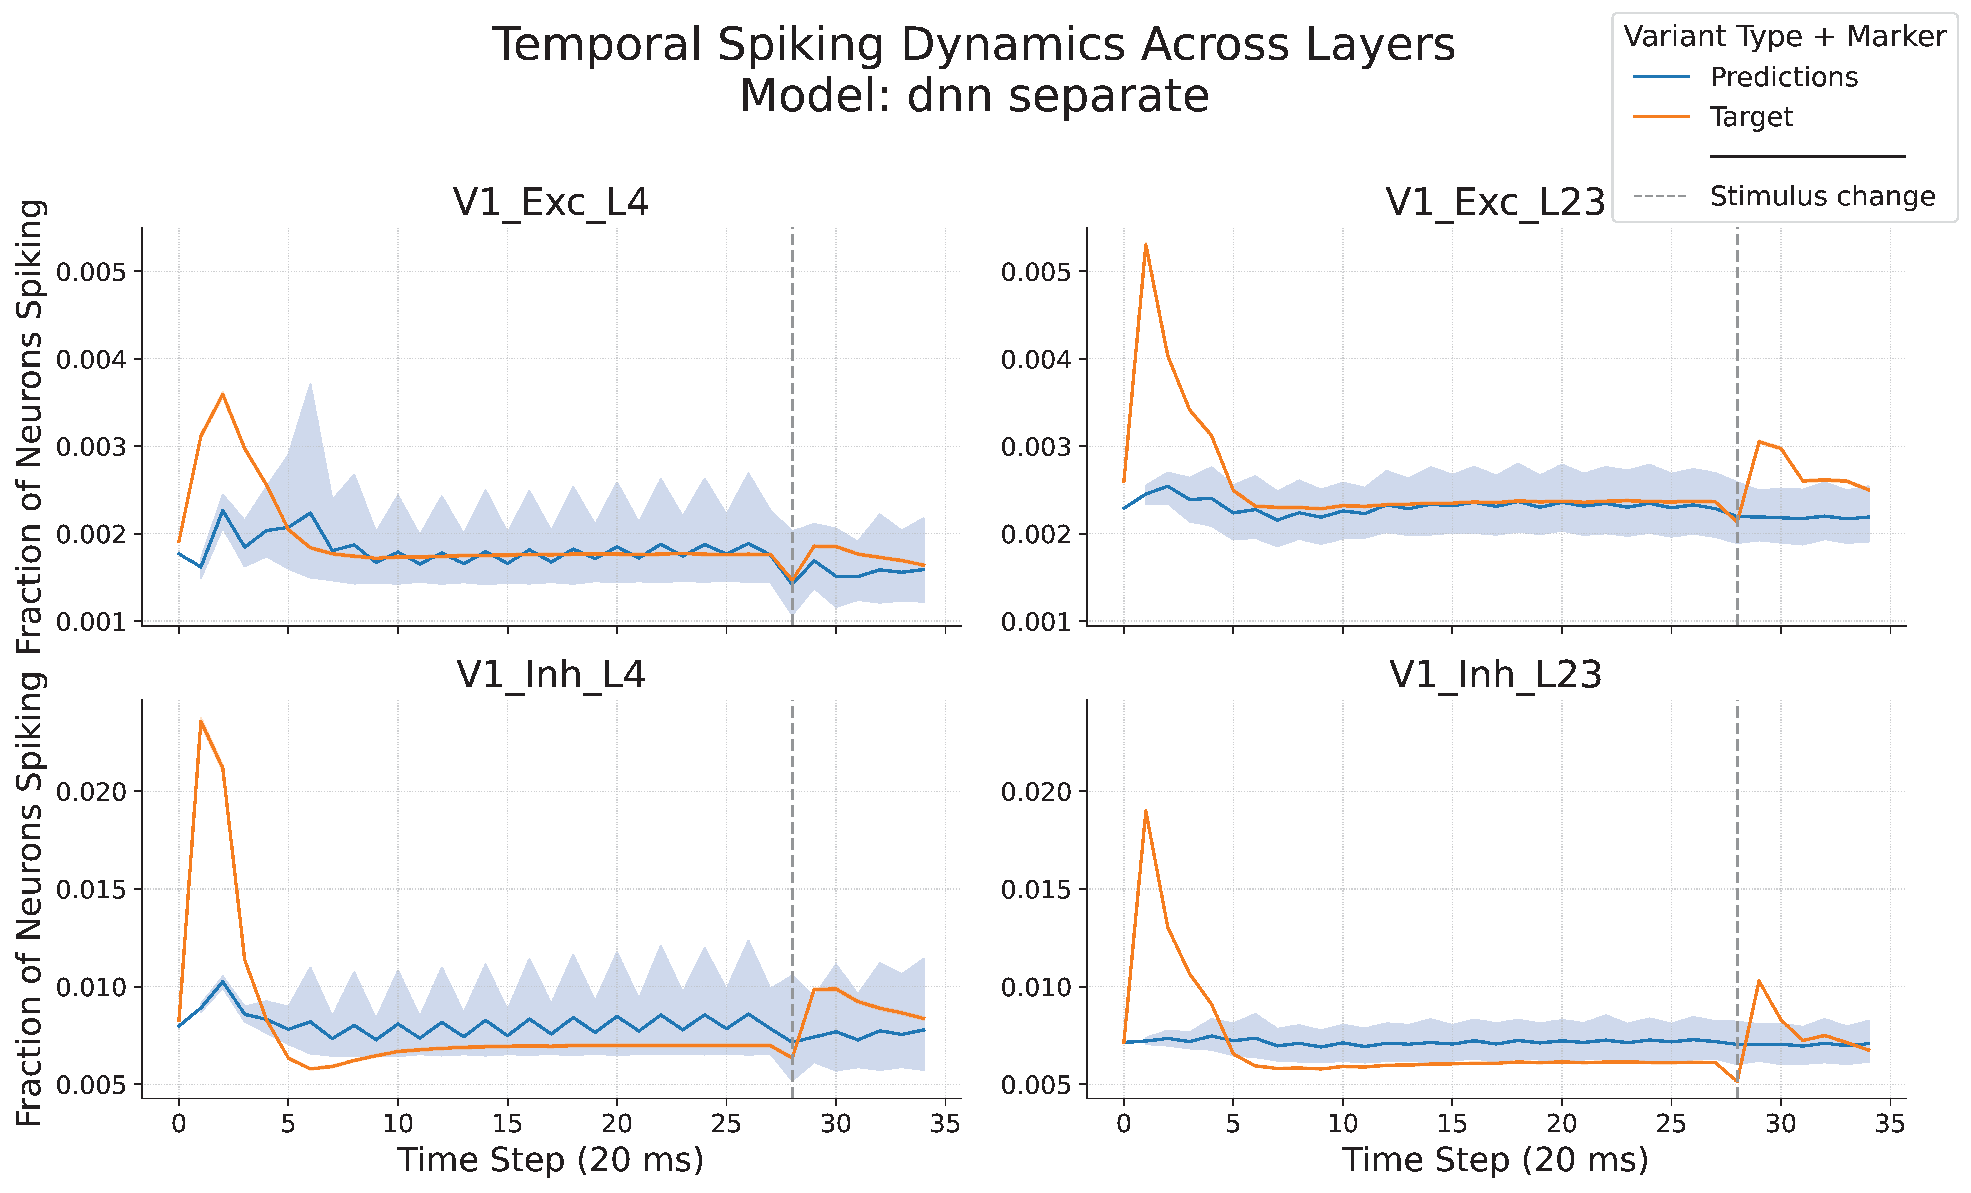
\includegraphics[width=\linewidth]{img/plots/separate_model_synchrony_curve_dnn_separate_evaluation.pdf}
    \caption{This figure depicts mean synchrony curve of dnn separate model predictions and its comparison to mean target synchrony curve both across all trials and all model subset variants including error bars. The dashed line marks the time step where the natural stimuli and blank stimuli changes.}
    \label{fig:synchrony_curve_dnn_separate}
\end{figure}

\subsubsection{RNN Separate Model With 5 Backpropagation Steps}
\label{{subsubsec:rnn_5_eval}}
\begin{figure}
    \centering
    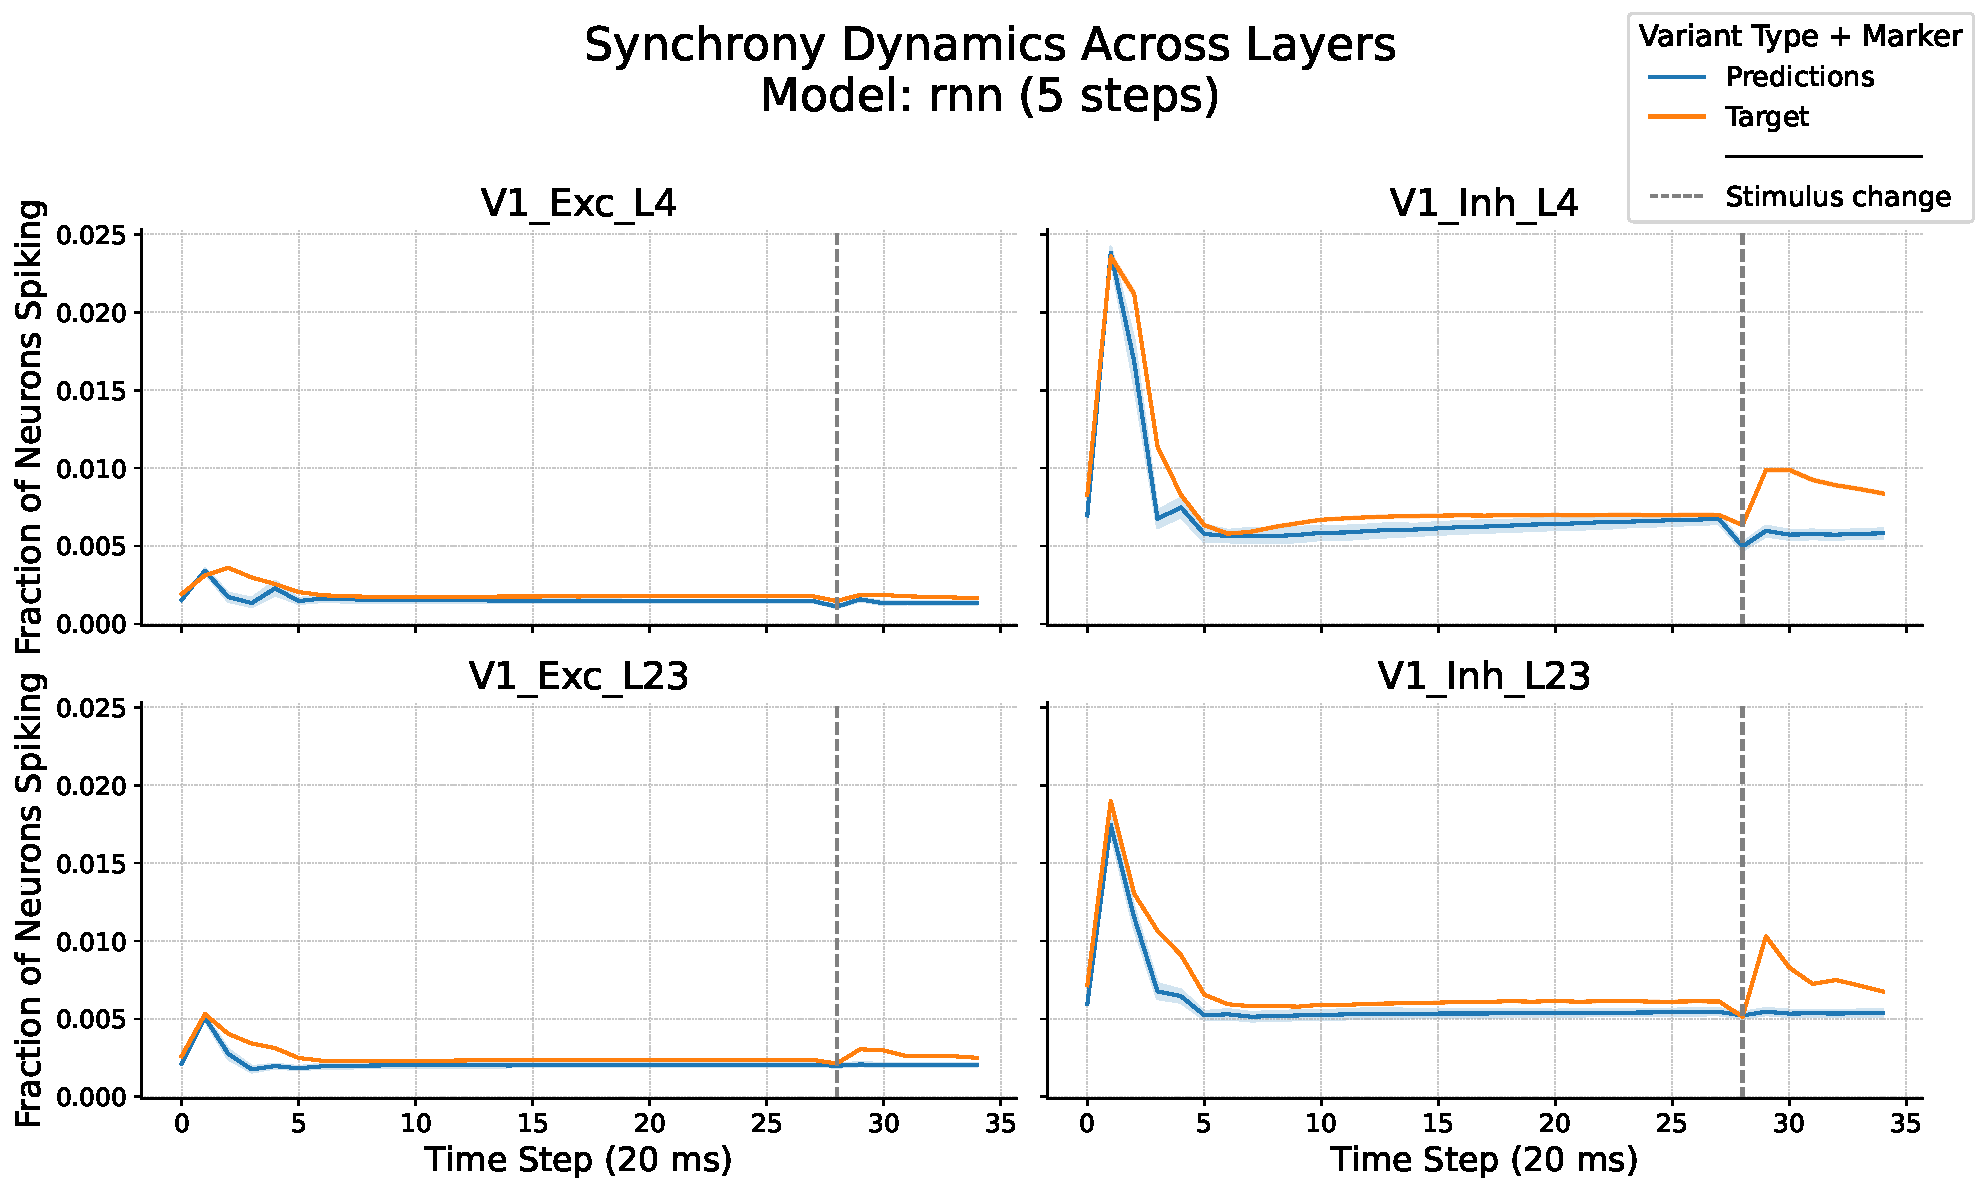
\includegraphics[width=\linewidth]{img/plots/separate_model_synchrony_curve_rnn_separate_5_evaluation.pdf}
    \caption{This figure depicts mean synchrony curve of rnn (time 5) model predictions and its comparison to mean target synchrony curve both across all trials and all model subset variants including error bars. The dashed line marks the time step where the natural stimuli and blank stimuli changes.}
    \label{fig:synchrony_curve_rnn_5}
\end{figure}


\subsubsection{RNN Separate Model With 10 Backpropagation Steps}
\label{{subsubsec:rnn_10_eval}}
\begin{figure}
    \centering
    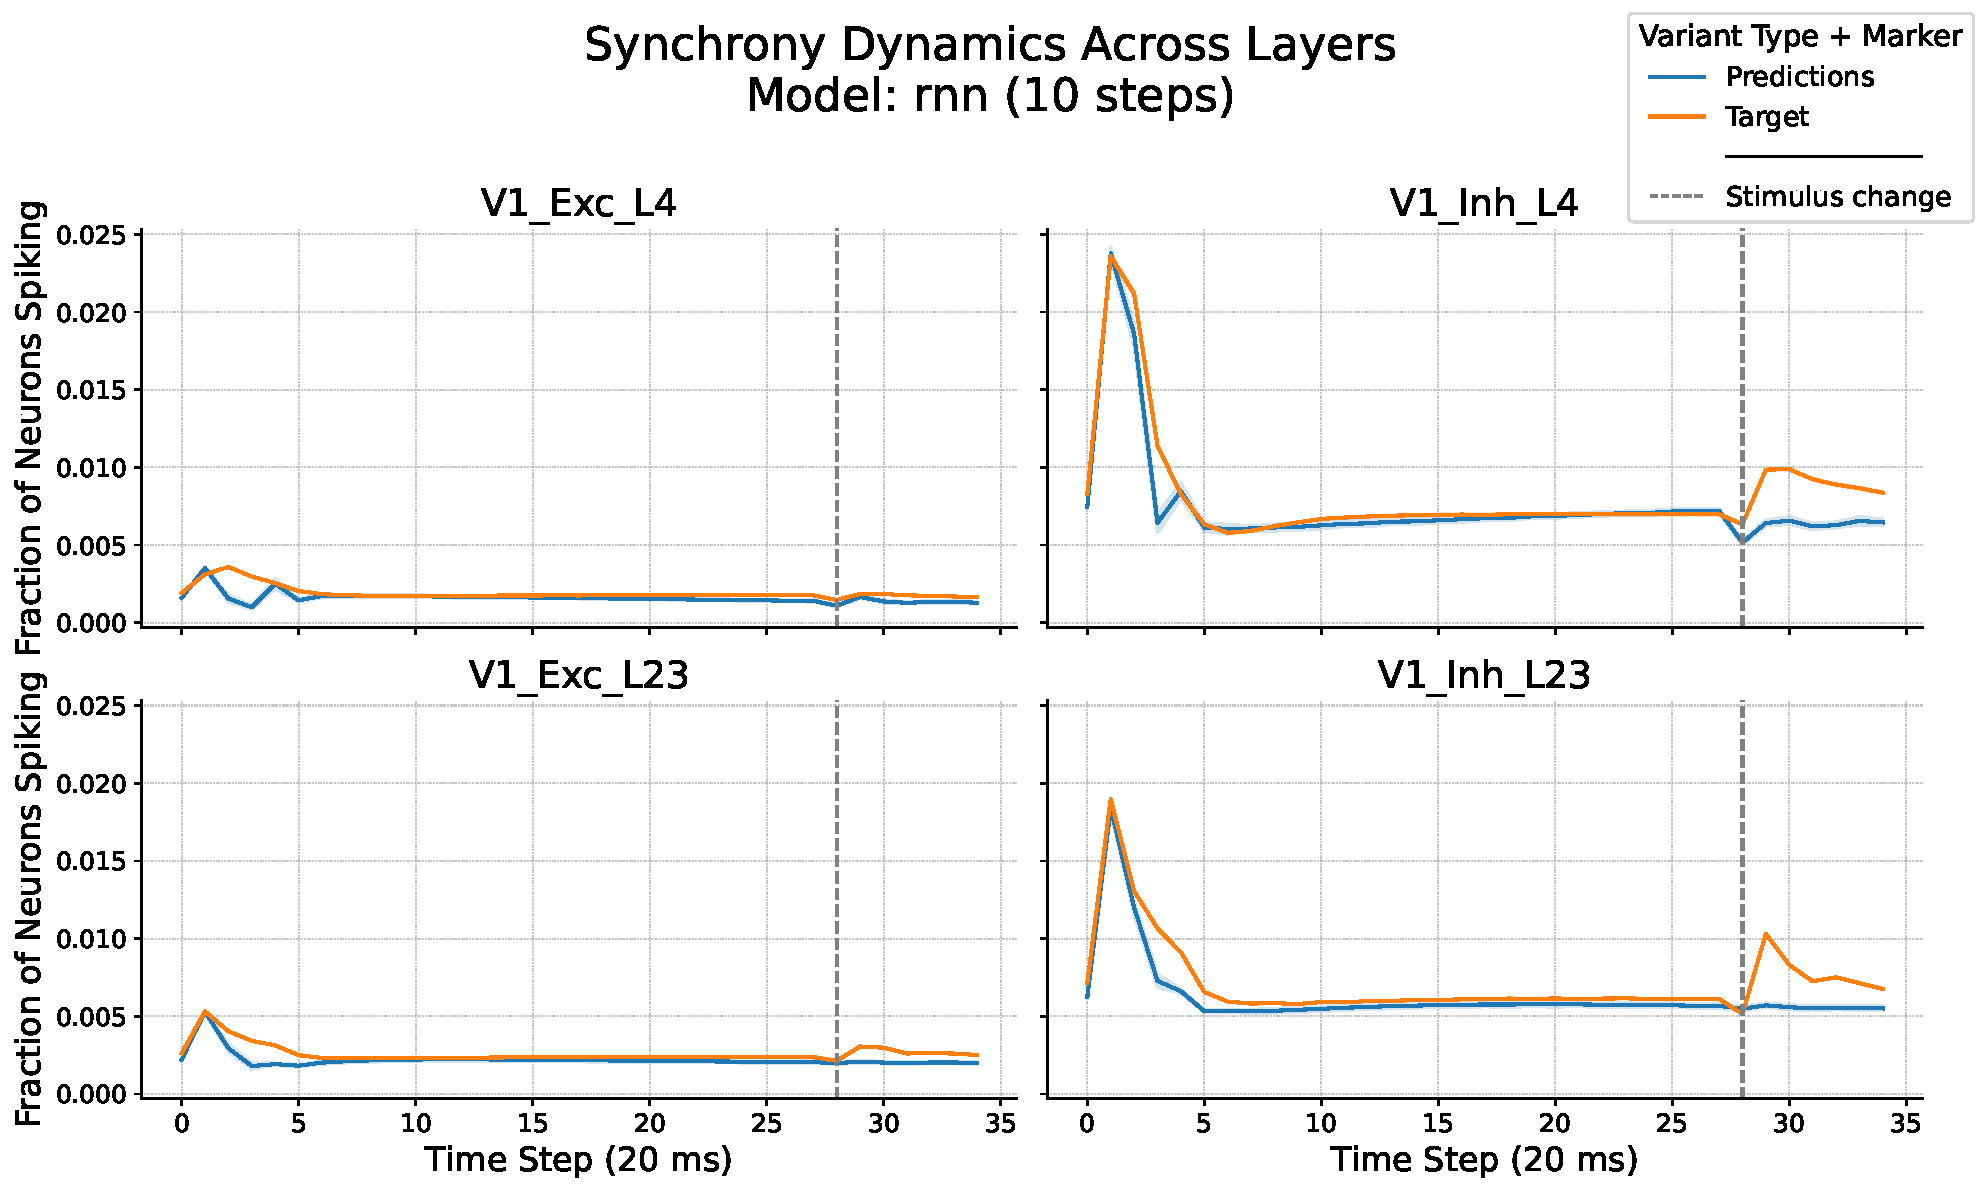
\includegraphics[width=\linewidth]{img/plots/separate_model_synchrony_curve_rnn_separate_10_evaluation.pdf}
    \caption{This figure depicts mean synchrony curve of rnn (time 10) model predictions and its comparison to mean target synchrony curve both across all trials and all model subset variants including error bars. The dashed line marks the time step where the natural stimuli and blank stimuli changes.}
    \label{fig:synchrony_curve_rnn_10}
\end{figure}

\subsubsection{Synpatic Depression Model Only On LGN with 5 Backpropagation Steps}
\label{{subsubsec:syn_adap_lgn_5}}
\begin{figure}
    \centering
    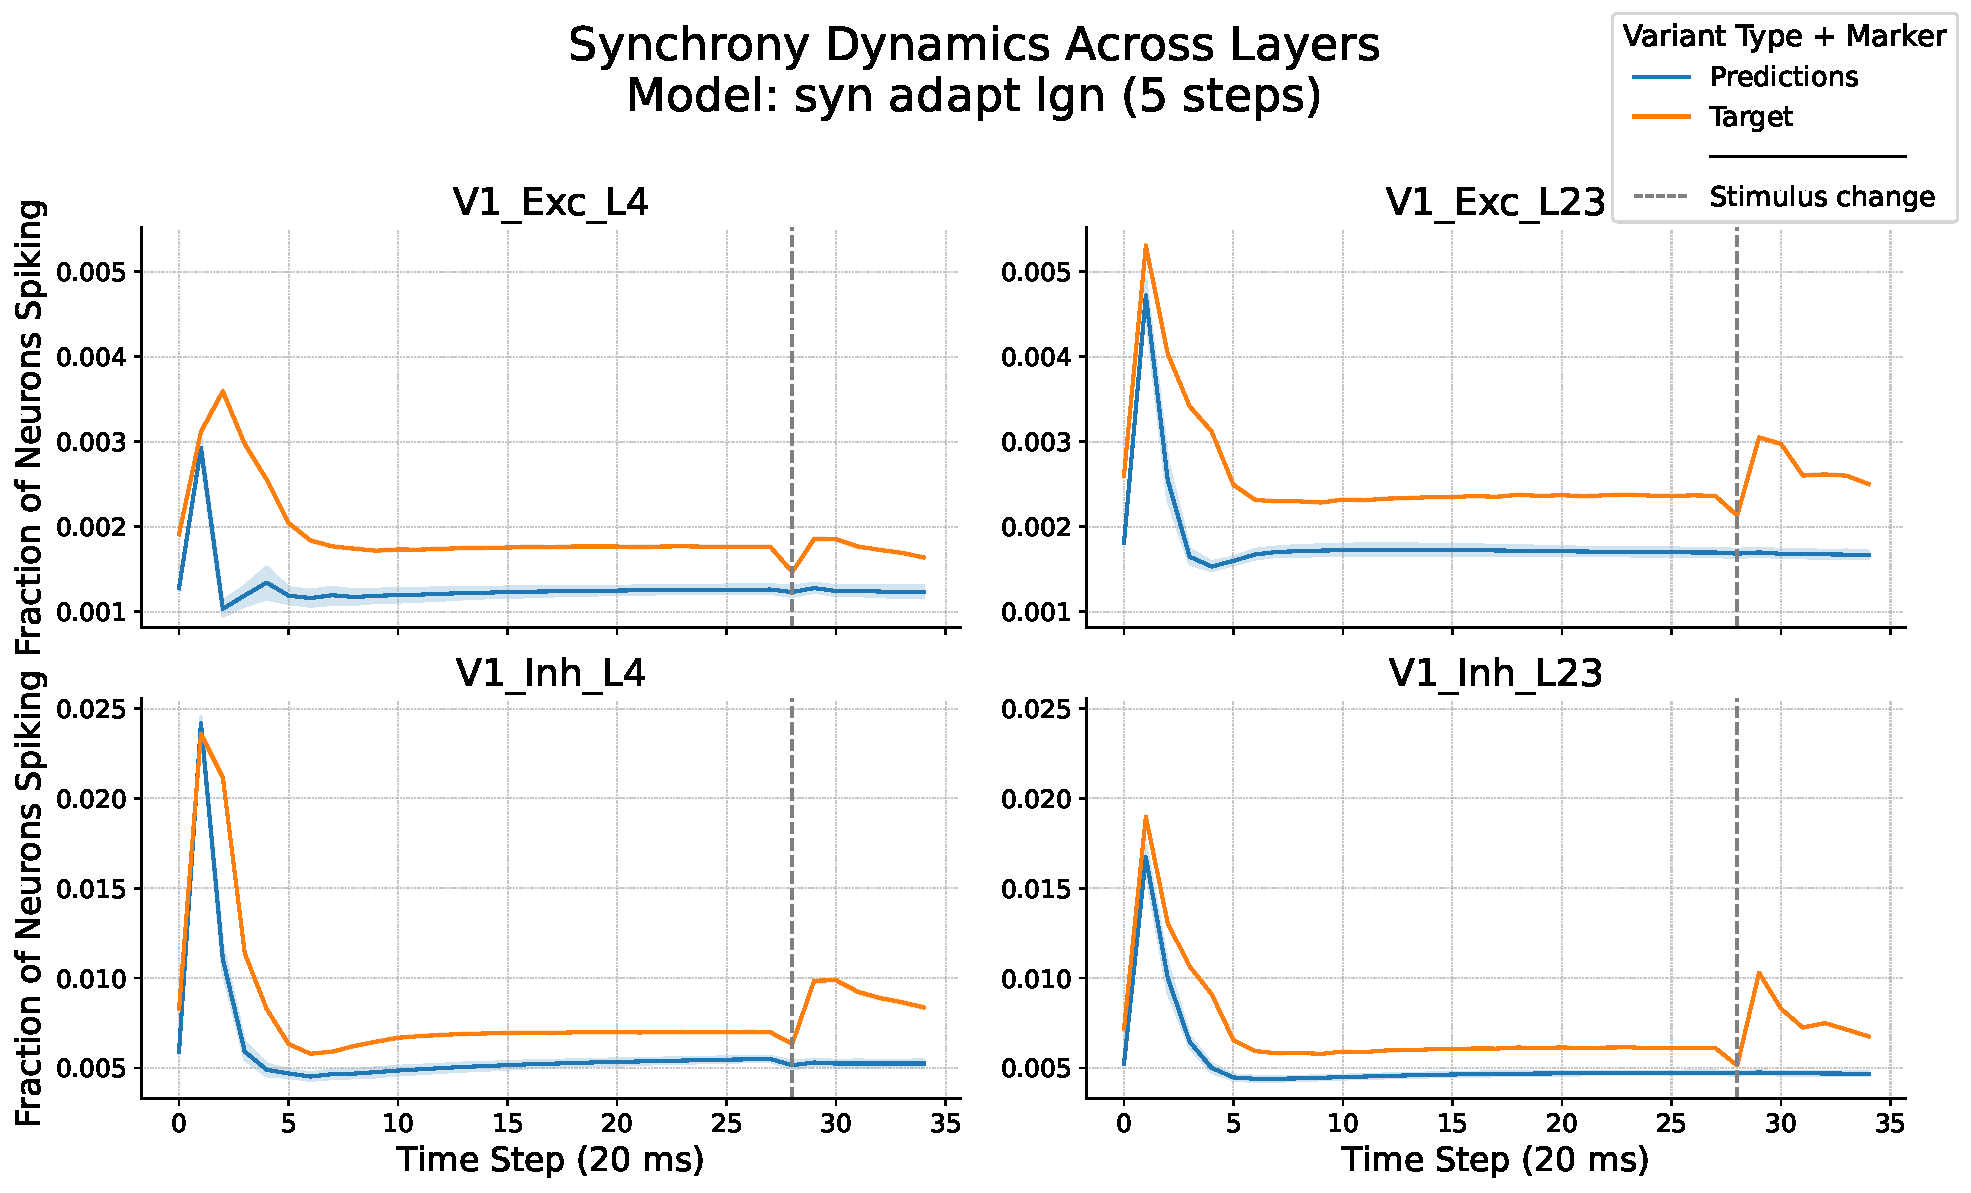
\includegraphics[width=\linewidth]{img/plots/separate_model_synchrony_curve_syn_only_lgn_5_evaluation.pdf}
    \caption{This figure depicts mean synchrony curve of syn adapt lgn (time 5) model predictions and its comparison to mean target synchrony curve both across all trials and all model subset variants including error bars. The dashed line marks the time step where the natural stimuli and blank stimuli changes.}
    \label{fig:synchrony_curve_syn_adapt_lgn_5}
\end{figure}

\section{Performance Gaps and Opportunities for Improvement}
\label{sec:performace_gaps_and_opportunities_for_improvement}
\subsection{Free vs Teacher-Forced Prediction Analysis}
\label{{subsec:free_vs_teacher_forced_predictions}}
\begin{figure}
    \centering
    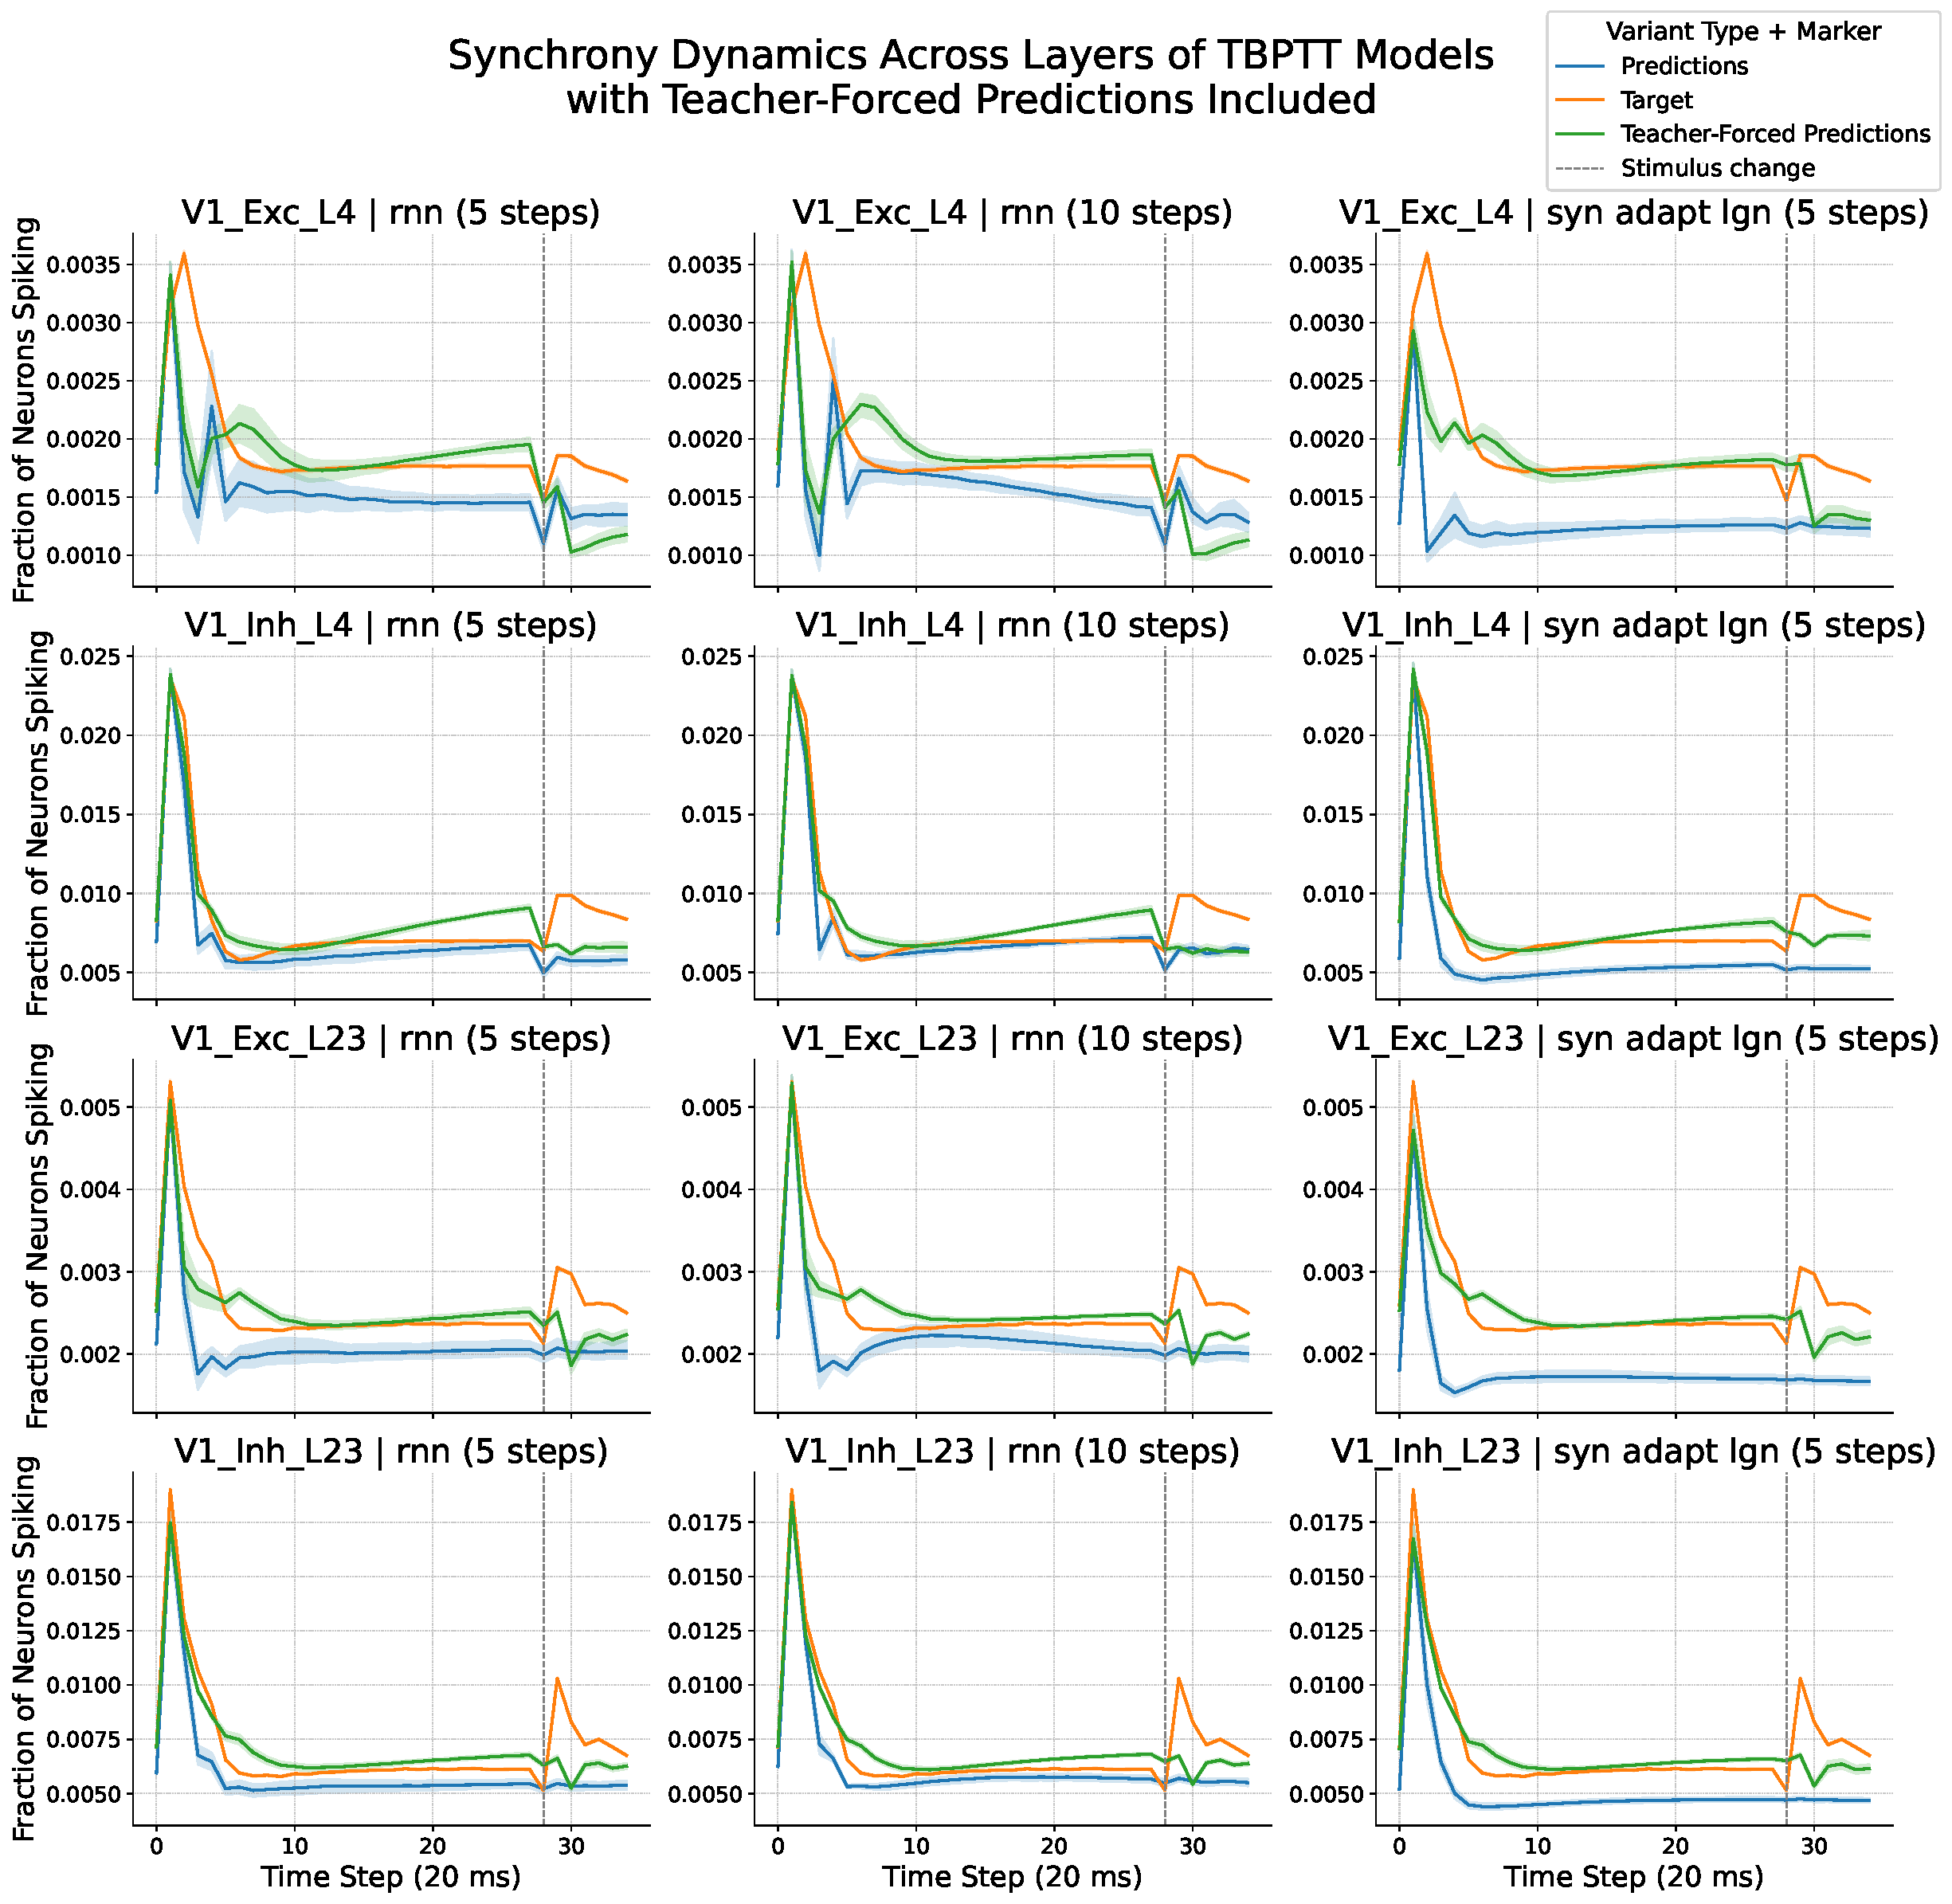
\includegraphics[width=\linewidth]{img/plots/tbptt_models_forced_included_model_synchrony_curve.pdf}
    \caption{This figure depicts mean synchrony curve of all model variants using TBPTT training algorithm. It depicts their predictions, teacher-forced predictions and its comparison to mean target synchrony curve both across all trials and all model subset variants including error bars. The dashed line marks the time step where the natural stimuli and blank stimuli changes.}
    \label{fig:free_vs_teacher_forced_synchrony}
\end{figure}

\begin{figure}
    \centering
    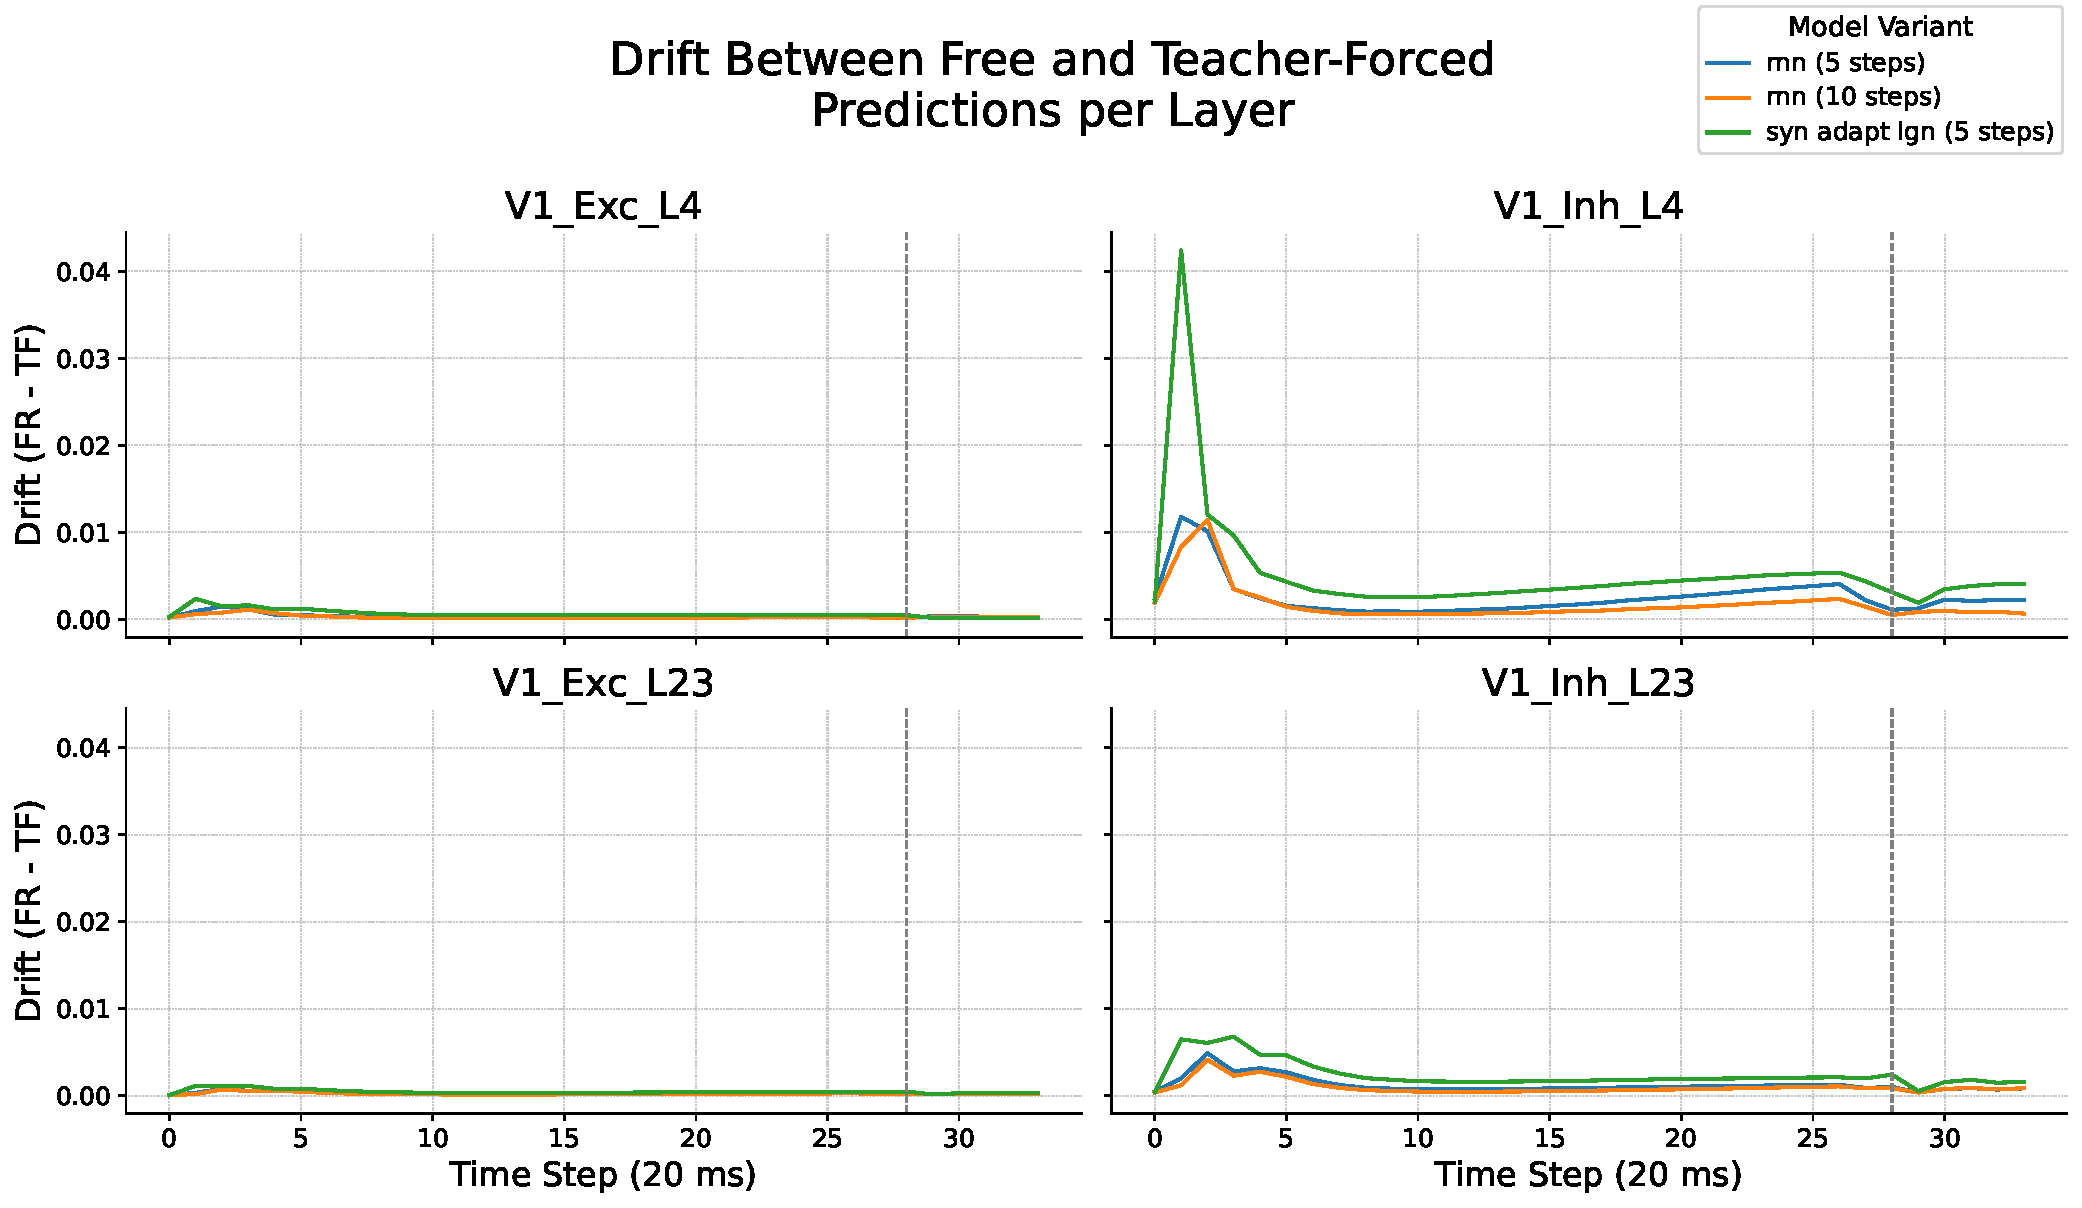
\includegraphics[width=\linewidth]{img/plots/temporal_drift_forced_free.pdf}
    \caption{}
    \label{fig:drift}
\end{figure}